
\subsection{Numerical solution}

In this section we present the numerical solution to problem
\eqref{eq:smith_hutton_cauchy_problem} for several values of the quotient $\rho
/ \Gamma$. So as to solve the problem numerically, the same \CC code has been
used as in the diagonal flow case only changing the boundary conditions and the
velocity field. It can be consulted
\href{https://github.com/plosan/convection_diffusion_equations}{here}.
The plots shown in this section have been produced with gnuplot 5.4. 

The characteristic length taken is $L = 1 \ \meter$. The density is
kept constant at $\rho = 1000 \ \kilo\gram / \meter^3$ and the diffusion
coefficient $\Gamma$ is varied. A uniform mesh has been used to discretize the
domain, with $N_x = 201$ nodes in the $x$--axis and $N_y = 101$ nodes in the
$y$--axis. The tolerance to stop Gauss--Seidel's iteration has been of
$10^{-12}$. The convective properties have been evaluated applying the
Power law Scheme. 

As it has been said, the characteristic length of the problem is $L = 1 \
\meter$, while the characteristic velocity is unknown. Nonetheless, it must be
constant as the velocity field $\vb{v}$ does not depend on time, hence Péclet's
number depends on the quotient $\rho / \Gamma$. This implies that $\rho /
\Gamma$ gives an idea of the relation convection transport rate/diffusion
transport rate.

Figure \ref{fig:smith_hutton_N201_Pe1.0e+00} shows the numerical solution to the
Smith--Hutton case for $\rho / \Gamma = 1$. Both processes, transport and
diffusion, apparently have a similar strength. There is clearly transport
phenomena taking the information about $\phi$ from the inlet zone $(-1, 0]
\times \{ 0 \}$ to the outlet zone $(0,1) \times \{ 0 \}$. For instance, the
inlet zone with $\phi \approx 1.0$ (green zone) occupies a rather small part of
the inlet around $x = -0.5 \ \meter$. However, as the transport occurs the band
corresponding to $\phi \approx 1$ becomes wider due to the diffusion process.
This influence of diffusion can also be ssen for $\phi \approx 0.5$ (light blue
band) and for $\phi \approx 1.5$ (orange band).

\begin{figure}[ht]
	\centering
	%	\fbox{% GNUPLOT: LaTeX picture with Postscript
\begingroup
  % Encoding inside the plot.  In the header of your document, this encoding
  % should to defined, e.g., by using
  % \usepackage[cp1252,<other encodings>]{inputenc}
  \inputencoding{cp1252}%
  \makeatletter
  \providecommand\color[2][]{%
    \GenericError{(gnuplot) \space\space\space\@spaces}{%
      Package color not loaded in conjunction with
      terminal option `colourtext'%
    }{See the gnuplot documentation for explanation.%
    }{Either use 'blacktext' in gnuplot or load the package
      color.sty in LaTeX.}%
    \renewcommand\color[2][]{}%
  }%
  \providecommand\includegraphics[2][]{%
    \GenericError{(gnuplot) \space\space\space\@spaces}{%
      Package graphicx or graphics not loaded%
    }{See the gnuplot documentation for explanation.%
    }{The gnuplot epslatex terminal needs graphicx.sty or graphics.sty.}%
    \renewcommand\includegraphics[2][]{}%
  }%
  \providecommand\rotatebox[2]{#2}%
  \@ifundefined{ifGPcolor}{%
    \newif\ifGPcolor
    \GPcolortrue
  }{}%
  \@ifundefined{ifGPblacktext}{%
    \newif\ifGPblacktext
    \GPblacktextfalse
  }{}%
  % define a \g@addto@macro without @ in the name:
  \let\gplgaddtomacro\g@addto@macro
  % define empty templates for all commands taking text:
  \gdef\gplbacktext{}%
  \gdef\gplfronttext{}%
  \makeatother
  \ifGPblacktext
    % no textcolor at all
    \def\colorrgb#1{}%
    \def\colorgray#1{}%
  \else
    % gray or color?
    \ifGPcolor
      \def\colorrgb#1{\color[rgb]{#1}}%
      \def\colorgray#1{\color[gray]{#1}}%
      \expandafter\def\csname LTw\endcsname{\color{white}}%
      \expandafter\def\csname LTb\endcsname{\color{black}}%
      \expandafter\def\csname LTa\endcsname{\color{black}}%
      \expandafter\def\csname LT0\endcsname{\color[rgb]{1,0,0}}%
      \expandafter\def\csname LT1\endcsname{\color[rgb]{0,1,0}}%
      \expandafter\def\csname LT2\endcsname{\color[rgb]{0,0,1}}%
      \expandafter\def\csname LT3\endcsname{\color[rgb]{1,0,1}}%
      \expandafter\def\csname LT4\endcsname{\color[rgb]{0,1,1}}%
      \expandafter\def\csname LT5\endcsname{\color[rgb]{1,1,0}}%
      \expandafter\def\csname LT6\endcsname{\color[rgb]{0,0,0}}%
      \expandafter\def\csname LT7\endcsname{\color[rgb]{1,0.3,0}}%
      \expandafter\def\csname LT8\endcsname{\color[rgb]{0.5,0.5,0.5}}%
    \else
      % gray
      \def\colorrgb#1{\color{black}}%
      \def\colorgray#1{\color[gray]{#1}}%
      \expandafter\def\csname LTw\endcsname{\color{white}}%
      \expandafter\def\csname LTb\endcsname{\color{black}}%
      \expandafter\def\csname LTa\endcsname{\color{black}}%
      \expandafter\def\csname LT0\endcsname{\color{black}}%
      \expandafter\def\csname LT1\endcsname{\color{black}}%
      \expandafter\def\csname LT2\endcsname{\color{black}}%
      \expandafter\def\csname LT3\endcsname{\color{black}}%
      \expandafter\def\csname LT4\endcsname{\color{black}}%
      \expandafter\def\csname LT5\endcsname{\color{black}}%
      \expandafter\def\csname LT6\endcsname{\color{black}}%
      \expandafter\def\csname LT7\endcsname{\color{black}}%
      \expandafter\def\csname LT8\endcsname{\color{black}}%
    \fi
  \fi
    \setlength{\unitlength}{0.0500bp}%
    \ifx\gptboxheight\undefined%
      \newlength{\gptboxheight}%
      \newlength{\gptboxwidth}%
      \newsavebox{\gptboxtext}%
    \fi%
    \setlength{\fboxrule}{0.5pt}%
    \setlength{\fboxsep}{1pt}%
    \definecolor{tbcol}{rgb}{1,1,1}%
\begin{picture}(7370.00,3968.00)%
    \gplgaddtomacro\gplbacktext{%
      \csname LTb\endcsname%%
      \put(814,719){\makebox(0,0)[r]{\strut{}0.0}}%
      \put(814,1234){\makebox(0,0)[r]{\strut{}0.2}}%
      \put(814,1748){\makebox(0,0)[r]{\strut{}0.4}}%
      \put(814,2263){\makebox(0,0)[r]{\strut{}0.6}}%
      \put(814,2777){\makebox(0,0)[r]{\strut{}0.8}}%
      \put(814,3292){\makebox(0,0)[r]{\strut{}1.0}}%
      \put(946,499){\makebox(0,0){\strut{}-1.0}}%
      \put(2233,499){\makebox(0,0){\strut{}-0.5}}%
      \put(3520,499){\makebox(0,0){\strut{}0.0}}%
      \put(4806,499){\makebox(0,0){\strut{}0.5}}%
      \put(6093,499){\makebox(0,0){\strut{}1.0}}%
    }%
    \gplgaddtomacro\gplfronttext{%
      \csname LTb\endcsname%%
      \put(209,2005){\rotatebox{-270}{\makebox(0,0){\strut{}$y \ (\mathrm{m})$}}}%
      \put(3519,169){\makebox(0,0){\strut{}$x \ (\mathrm{m})$}}%
      \csname LTb\endcsname%%
      \put(6611,719){\makebox(0,0)[l]{\strut{}0.0}}%
      \put(6611,1362){\makebox(0,0)[l]{\strut{}0.5}}%
      \put(6611,2005){\makebox(0,0)[l]{\strut{}1.0}}%
      \put(6611,2648){\makebox(0,0)[l]{\strut{}1.5}}%
      \put(6611,3292){\makebox(0,0)[l]{\strut{}2.0}}%
      \put(7073,2005){\rotatebox{-270}{\makebox(0,0){\strut{}$\phi$}}}%
      \put(3519,3622){\makebox(0,0){\strut{}\textbf{Smith--Hutton case} $(\mathrm{Pe} = 1)$}}%
    }%
    \gplbacktext
    \put(0,0){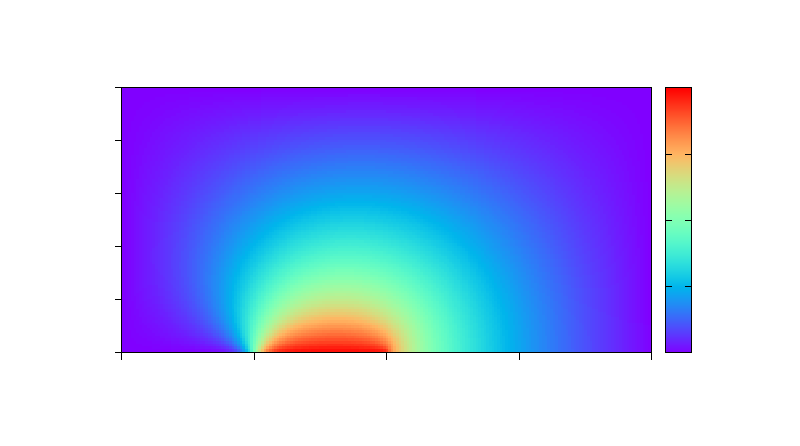
\includegraphics[width={368.50bp},height={198.40bp}]{figures/case_smith_hutton/smith_hutton_N201_Pe1.0e+00}}%
    \gplfronttext
  \end{picture}%
\endgroup
}
	% GNUPLOT: LaTeX picture with Postscript
\begingroup
  % Encoding inside the plot.  In the header of your document, this encoding
  % should to defined, e.g., by using
  % \usepackage[cp1252,<other encodings>]{inputenc}
  \inputencoding{cp1252}%
  \makeatletter
  \providecommand\color[2][]{%
    \GenericError{(gnuplot) \space\space\space\@spaces}{%
      Package color not loaded in conjunction with
      terminal option `colourtext'%
    }{See the gnuplot documentation for explanation.%
    }{Either use 'blacktext' in gnuplot or load the package
      color.sty in LaTeX.}%
    \renewcommand\color[2][]{}%
  }%
  \providecommand\includegraphics[2][]{%
    \GenericError{(gnuplot) \space\space\space\@spaces}{%
      Package graphicx or graphics not loaded%
    }{See the gnuplot documentation for explanation.%
    }{The gnuplot epslatex terminal needs graphicx.sty or graphics.sty.}%
    \renewcommand\includegraphics[2][]{}%
  }%
  \providecommand\rotatebox[2]{#2}%
  \@ifundefined{ifGPcolor}{%
    \newif\ifGPcolor
    \GPcolortrue
  }{}%
  \@ifundefined{ifGPblacktext}{%
    \newif\ifGPblacktext
    \GPblacktextfalse
  }{}%
  % define a \g@addto@macro without @ in the name:
  \let\gplgaddtomacro\g@addto@macro
  % define empty templates for all commands taking text:
  \gdef\gplbacktext{}%
  \gdef\gplfronttext{}%
  \makeatother
  \ifGPblacktext
    % no textcolor at all
    \def\colorrgb#1{}%
    \def\colorgray#1{}%
  \else
    % gray or color?
    \ifGPcolor
      \def\colorrgb#1{\color[rgb]{#1}}%
      \def\colorgray#1{\color[gray]{#1}}%
      \expandafter\def\csname LTw\endcsname{\color{white}}%
      \expandafter\def\csname LTb\endcsname{\color{black}}%
      \expandafter\def\csname LTa\endcsname{\color{black}}%
      \expandafter\def\csname LT0\endcsname{\color[rgb]{1,0,0}}%
      \expandafter\def\csname LT1\endcsname{\color[rgb]{0,1,0}}%
      \expandafter\def\csname LT2\endcsname{\color[rgb]{0,0,1}}%
      \expandafter\def\csname LT3\endcsname{\color[rgb]{1,0,1}}%
      \expandafter\def\csname LT4\endcsname{\color[rgb]{0,1,1}}%
      \expandafter\def\csname LT5\endcsname{\color[rgb]{1,1,0}}%
      \expandafter\def\csname LT6\endcsname{\color[rgb]{0,0,0}}%
      \expandafter\def\csname LT7\endcsname{\color[rgb]{1,0.3,0}}%
      \expandafter\def\csname LT8\endcsname{\color[rgb]{0.5,0.5,0.5}}%
    \else
      % gray
      \def\colorrgb#1{\color{black}}%
      \def\colorgray#1{\color[gray]{#1}}%
      \expandafter\def\csname LTw\endcsname{\color{white}}%
      \expandafter\def\csname LTb\endcsname{\color{black}}%
      \expandafter\def\csname LTa\endcsname{\color{black}}%
      \expandafter\def\csname LT0\endcsname{\color{black}}%
      \expandafter\def\csname LT1\endcsname{\color{black}}%
      \expandafter\def\csname LT2\endcsname{\color{black}}%
      \expandafter\def\csname LT3\endcsname{\color{black}}%
      \expandafter\def\csname LT4\endcsname{\color{black}}%
      \expandafter\def\csname LT5\endcsname{\color{black}}%
      \expandafter\def\csname LT6\endcsname{\color{black}}%
      \expandafter\def\csname LT7\endcsname{\color{black}}%
      \expandafter\def\csname LT8\endcsname{\color{black}}%
    \fi
  \fi
    \setlength{\unitlength}{0.0500bp}%
    \ifx\gptboxheight\undefined%
      \newlength{\gptboxheight}%
      \newlength{\gptboxwidth}%
      \newsavebox{\gptboxtext}%
    \fi%
    \setlength{\fboxrule}{0.5pt}%
    \setlength{\fboxsep}{1pt}%
    \definecolor{tbcol}{rgb}{1,1,1}%
\begin{picture}(7370.00,3968.00)%
    \gplgaddtomacro\gplbacktext{%
      \csname LTb\endcsname%%
      \put(814,719){\makebox(0,0)[r]{\strut{}0.0}}%
      \put(814,1234){\makebox(0,0)[r]{\strut{}0.2}}%
      \put(814,1748){\makebox(0,0)[r]{\strut{}0.4}}%
      \put(814,2263){\makebox(0,0)[r]{\strut{}0.6}}%
      \put(814,2777){\makebox(0,0)[r]{\strut{}0.8}}%
      \put(814,3292){\makebox(0,0)[r]{\strut{}1.0}}%
      \put(946,499){\makebox(0,0){\strut{}-1.0}}%
      \put(2233,499){\makebox(0,0){\strut{}-0.5}}%
      \put(3520,499){\makebox(0,0){\strut{}0.0}}%
      \put(4806,499){\makebox(0,0){\strut{}0.5}}%
      \put(6093,499){\makebox(0,0){\strut{}1.0}}%
    }%
    \gplgaddtomacro\gplfronttext{%
      \csname LTb\endcsname%%
      \put(209,2005){\rotatebox{-270}{\makebox(0,0){\strut{}$y \ (\mathrm{m})$}}}%
      \put(3519,169){\makebox(0,0){\strut{}$x \ (\mathrm{m})$}}%
      \csname LTb\endcsname%%
      \put(6611,719){\makebox(0,0)[l]{\strut{}0.0}}%
      \put(6611,1362){\makebox(0,0)[l]{\strut{}0.5}}%
      \put(6611,2005){\makebox(0,0)[l]{\strut{}1.0}}%
      \put(6611,2648){\makebox(0,0)[l]{\strut{}1.5}}%
      \put(6611,3292){\makebox(0,0)[l]{\strut{}2.0}}%
      \put(7073,2005){\rotatebox{-270}{\makebox(0,0){\strut{}$\phi$}}}%
      \put(3519,3622){\makebox(0,0){\strut{}\textbf{Smith--Hutton case} $(\mathrm{Pe} = 1)$}}%
    }%
    \gplbacktext
    \put(0,0){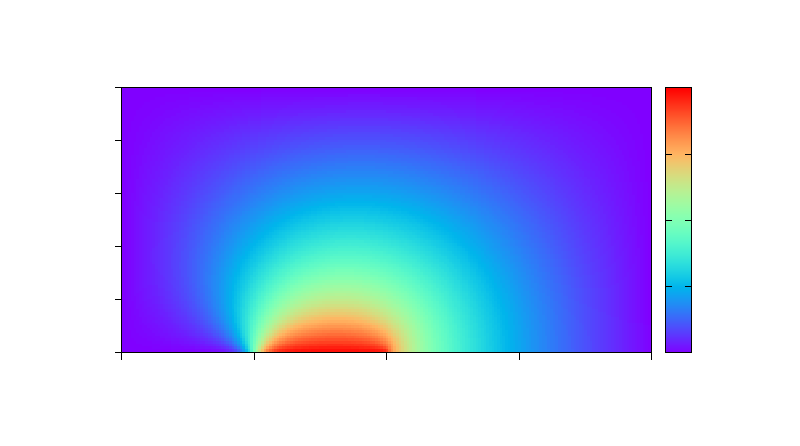
\includegraphics[width={368.50bp},height={198.40bp}]{figures/case_smith_hutton/smith_hutton_N201_Pe1.0e+00}}%
    \gplfronttext
  \end{picture}%
\endgroup

	\caption{Numerical solution the the Smith--Hutton case for $\rho / \Gamma = 1$.}
	\label{fig:smith_hutton_N201_Pe1.0e+00}
\end{figure}

\clearpage
Figures \ref{fig:smith_hutton_N201_Pe1.0e+01} and
\ref{fig:smith_hutton_N201_Pe1.0e+02} show the numerical solution to the
Smith--Hutton problem for $\rho / \Gamma = 10$ and $\rho / \Gamma = 100$,
respectively. Some differences between the solutions for $\rho / \Gamma = 1$ and
$\rho / \Gamma = 10$, although not too obvious, can be spotted. Clearly the
light blue, green and orange bands now occupy a larger portion of $\Omega$,
while the smooth transitions between them are still present. In contrast to the
$\rho / \Gamma = 10$ case, the change for $\rho / \Gamma = 100$ is more
apparent. Now the transition zones between the different color bands are
thinner, implying the diffusion process has lost strength with respect to the
transport process. However there is still diffusion, since the green band widens
along the streamlines.

\begin{figure}[ht]
	\centering
	%	\fbox{% GNUPLOT: LaTeX picture with Postscript
\documentclass{minimal}
% Set font size
\makeatletter
\def\@ptsize{1}
\InputIfFileExists{size11.clo}{}{%
   \GenericError{(gnuplot) \space\space\space\@spaces}{%
      Gnuplot Error: File `size11.clo' not found! Could not set font size%
   }{See the gnuplot documentation for explanation.%
   }{For using a font size a file `size<fontsize>.clo' has to exist.
        Falling back ^^Jto default fontsize 10pt.}%
  \def\@ptsize{0}
  \input{size10.clo}%
}%
\makeatother
% Load packages
\usepackage{calc}
\usepackage{graphicx}
\usepackage{color}
\usepackage[cp1252]{inputenc}
\makeatletter
% Select an appropriate default driver (from TeXLive graphics.cfg)
\begingroup
  \chardef\x=0 %
  % check pdfTeX
  \@ifundefined{pdfoutput}{}{%
    \ifcase\pdfoutput
    \else
      \chardef\x=1 %
    \fi
  }%
  % check VTeX
  \@ifundefined{OpMode}{}{%
    \chardef\x=2 %
  }%
\expandafter\endgroup
\ifcase\x
  % default case
  \PassOptionsToPackage{dvips}{geometry}
\or
  % pdfTeX is running in pdf mode
  \PassOptionsToPackage{pdftex}{geometry}
\else
  % VTeX is running
  \PassOptionsToPackage{vtex}{geometry}
\fi
\makeatother
% Set papersize
\usepackage[papersize={368.50bp,198.40bp},text={368.50bp,198.40bp}]{geometry}
% No page numbers and no paragraph indentation
\pagestyle{empty}
\setlength{\parindent}{0bp}%
% Load configuration file
\InputIfFileExists{gnuplot.cfg}{%
  \typeout{Using configuration file gnuplot.cfg}%
}{%
 \typeout{No configuration file gnuplot.cfg found.}%
}%
%
\begin{document}
\begingroup
  % Encoding inside the plot.  In the header of your document, this encoding
  % should to defined, e.g., by using
  % \usepackage[cp1252,<other encodings>]{inputenc}
  \inputencoding{cp1252}%
  \makeatletter
  \providecommand\color[2][]{%
    \GenericError{(gnuplot) \space\space\space\@spaces}{%
      Package color not loaded in conjunction with
      terminal option `colourtext'%
    }{See the gnuplot documentation for explanation.%
    }{Either use 'blacktext' in gnuplot or load the package
      color.sty in LaTeX.}%
    \renewcommand\color[2][]{}%
  }%
  \providecommand\includegraphics[2][]{%
    \GenericError{(gnuplot) \space\space\space\@spaces}{%
      Package graphicx or graphics not loaded%
    }{See the gnuplot documentation for explanation.%
    }{The gnuplot epslatex terminal needs graphicx.sty or graphics.sty.}%
    \renewcommand\includegraphics[2][]{}%
  }%
  \providecommand\rotatebox[2]{#2}%
  \@ifundefined{ifGPcolor}{%
    \newif\ifGPcolor
    \GPcolortrue
  }{}%
  \@ifundefined{ifGPblacktext}{%
    \newif\ifGPblacktext
    \GPblacktextfalse
  }{}%
  % define a \g@addto@macro without @ in the name:
  \let\gplgaddtomacro\g@addto@macro
  % define empty templates for all commands taking text:
  \gdef\gplbacktext{}%
  \gdef\gplfronttext{}%
  \makeatother
  \ifGPblacktext
    % no textcolor at all
    \def\colorrgb#1{}%
    \def\colorgray#1{}%
  \else
    % gray or color?
    \ifGPcolor
      \def\colorrgb#1{\color[rgb]{#1}}%
      \def\colorgray#1{\color[gray]{#1}}%
      \expandafter\def\csname LTw\endcsname{\color{white}}%
      \expandafter\def\csname LTb\endcsname{\color{black}}%
      \expandafter\def\csname LTa\endcsname{\color{black}}%
      \expandafter\def\csname LT0\endcsname{\color[rgb]{1,0,0}}%
      \expandafter\def\csname LT1\endcsname{\color[rgb]{0,1,0}}%
      \expandafter\def\csname LT2\endcsname{\color[rgb]{0,0,1}}%
      \expandafter\def\csname LT3\endcsname{\color[rgb]{1,0,1}}%
      \expandafter\def\csname LT4\endcsname{\color[rgb]{0,1,1}}%
      \expandafter\def\csname LT5\endcsname{\color[rgb]{1,1,0}}%
      \expandafter\def\csname LT6\endcsname{\color[rgb]{0,0,0}}%
      \expandafter\def\csname LT7\endcsname{\color[rgb]{1,0.3,0}}%
      \expandafter\def\csname LT8\endcsname{\color[rgb]{0.5,0.5,0.5}}%
    \else
      % gray
      \def\colorrgb#1{\color{black}}%
      \def\colorgray#1{\color[gray]{#1}}%
      \expandafter\def\csname LTw\endcsname{\color{white}}%
      \expandafter\def\csname LTb\endcsname{\color{black}}%
      \expandafter\def\csname LTa\endcsname{\color{black}}%
      \expandafter\def\csname LT0\endcsname{\color{black}}%
      \expandafter\def\csname LT1\endcsname{\color{black}}%
      \expandafter\def\csname LT2\endcsname{\color{black}}%
      \expandafter\def\csname LT3\endcsname{\color{black}}%
      \expandafter\def\csname LT4\endcsname{\color{black}}%
      \expandafter\def\csname LT5\endcsname{\color{black}}%
      \expandafter\def\csname LT6\endcsname{\color{black}}%
      \expandafter\def\csname LT7\endcsname{\color{black}}%
      \expandafter\def\csname LT8\endcsname{\color{black}}%
    \fi
  \fi
    \setlength{\unitlength}{0.0500bp}%
    \ifx\gptboxheight\undefined%
      \newlength{\gptboxheight}%
      \newlength{\gptboxwidth}%
      \newsavebox{\gptboxtext}%
    \fi%
    \setlength{\fboxrule}{0.5pt}%
    \setlength{\fboxsep}{1pt}%
    \definecolor{tbcol}{rgb}{1,1,1}%
\begin{picture}(7370.00,3968.00)%
    \gplgaddtomacro\gplbacktext{%
      \csname LTb\endcsname%%
      \put(814,733){\makebox(0,0)[r]{\strut{}0.0}}%
      \put(814,1242){\makebox(0,0)[r]{\strut{}0.2}}%
      \put(814,1751){\makebox(0,0)[r]{\strut{}0.4}}%
      \put(814,2260){\makebox(0,0)[r]{\strut{}0.6}}%
      \put(814,2769){\makebox(0,0)[r]{\strut{}0.8}}%
      \put(814,3278){\makebox(0,0)[r]{\strut{}1.0}}%
      \put(1009,513){\makebox(0,0){\strut{}-1.0}}%
      \put(2282,513){\makebox(0,0){\strut{}-0.5}}%
      \put(3554,513){\makebox(0,0){\strut{}0.0}}%
      \put(4827,513){\makebox(0,0){\strut{}0.5}}%
      \put(6099,513){\makebox(0,0){\strut{}1.0}}%
    }%
    \gplgaddtomacro\gplfronttext{%
      \csname LTb\endcsname%%
      \put(209,2005){\rotatebox{-270}{\makebox(0,0){\strut{}$y \ (\mathrm{m})$}}}%
      \put(3554,183){\makebox(0,0){\strut{}$x \ (\mathrm{m})$}}%
      \csname LTb\endcsname%%
      \put(6612,733){\makebox(0,0)[l]{\strut{}0.0}}%
      \put(6612,1369){\makebox(0,0)[l]{\strut{}0.5}}%
      \put(6612,2005){\makebox(0,0)[l]{\strut{}1.0}}%
      \put(6612,2641){\makebox(0,0)[l]{\strut{}1.5}}%
      \put(6612,3278){\makebox(0,0)[l]{\strut{}2.0}}%
      \put(7074,2005){\rotatebox{-270}{\makebox(0,0){\strut{}$\phi$}}}%
      \put(3554,3608){\makebox(0,0){\strut{}\textbf{Smith--Hutton case} $(\rho / \Gamma = 10)$}}%
    }%
    \gplbacktext
    \put(0,0){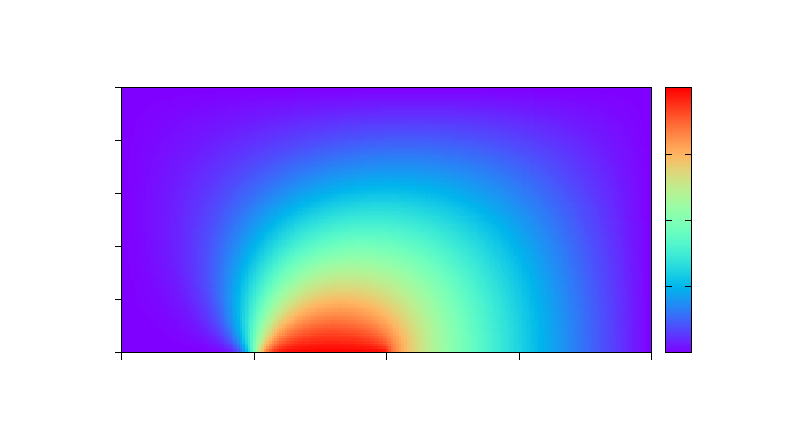
\includegraphics[width={368.50bp},height={198.40bp}]{smith_hutton_N201_Pe1.0e+01-inc}}%
    \gplfronttext
  \end{picture}%
\endgroup
\end{document}
}
	% GNUPLOT: LaTeX picture with Postscript
\documentclass{minimal}
% Set font size
\makeatletter
\def\@ptsize{1}
\InputIfFileExists{size11.clo}{}{%
   \GenericError{(gnuplot) \space\space\space\@spaces}{%
      Gnuplot Error: File `size11.clo' not found! Could not set font size%
   }{See the gnuplot documentation for explanation.%
   }{For using a font size a file `size<fontsize>.clo' has to exist.
        Falling back ^^Jto default fontsize 10pt.}%
  \def\@ptsize{0}
  \input{size10.clo}%
}%
\makeatother
% Load packages
\usepackage{calc}
\usepackage{graphicx}
\usepackage{color}
\usepackage[cp1252]{inputenc}
\makeatletter
% Select an appropriate default driver (from TeXLive graphics.cfg)
\begingroup
  \chardef\x=0 %
  % check pdfTeX
  \@ifundefined{pdfoutput}{}{%
    \ifcase\pdfoutput
    \else
      \chardef\x=1 %
    \fi
  }%
  % check VTeX
  \@ifundefined{OpMode}{}{%
    \chardef\x=2 %
  }%
\expandafter\endgroup
\ifcase\x
  % default case
  \PassOptionsToPackage{dvips}{geometry}
\or
  % pdfTeX is running in pdf mode
  \PassOptionsToPackage{pdftex}{geometry}
\else
  % VTeX is running
  \PassOptionsToPackage{vtex}{geometry}
\fi
\makeatother
% Set papersize
\usepackage[papersize={368.50bp,198.40bp},text={368.50bp,198.40bp}]{geometry}
% No page numbers and no paragraph indentation
\pagestyle{empty}
\setlength{\parindent}{0bp}%
% Load configuration file
\InputIfFileExists{gnuplot.cfg}{%
  \typeout{Using configuration file gnuplot.cfg}%
}{%
 \typeout{No configuration file gnuplot.cfg found.}%
}%
%
\begin{document}
\begingroup
  % Encoding inside the plot.  In the header of your document, this encoding
  % should to defined, e.g., by using
  % \usepackage[cp1252,<other encodings>]{inputenc}
  \inputencoding{cp1252}%
  \makeatletter
  \providecommand\color[2][]{%
    \GenericError{(gnuplot) \space\space\space\@spaces}{%
      Package color not loaded in conjunction with
      terminal option `colourtext'%
    }{See the gnuplot documentation for explanation.%
    }{Either use 'blacktext' in gnuplot or load the package
      color.sty in LaTeX.}%
    \renewcommand\color[2][]{}%
  }%
  \providecommand\includegraphics[2][]{%
    \GenericError{(gnuplot) \space\space\space\@spaces}{%
      Package graphicx or graphics not loaded%
    }{See the gnuplot documentation for explanation.%
    }{The gnuplot epslatex terminal needs graphicx.sty or graphics.sty.}%
    \renewcommand\includegraphics[2][]{}%
  }%
  \providecommand\rotatebox[2]{#2}%
  \@ifundefined{ifGPcolor}{%
    \newif\ifGPcolor
    \GPcolortrue
  }{}%
  \@ifundefined{ifGPblacktext}{%
    \newif\ifGPblacktext
    \GPblacktextfalse
  }{}%
  % define a \g@addto@macro without @ in the name:
  \let\gplgaddtomacro\g@addto@macro
  % define empty templates for all commands taking text:
  \gdef\gplbacktext{}%
  \gdef\gplfronttext{}%
  \makeatother
  \ifGPblacktext
    % no textcolor at all
    \def\colorrgb#1{}%
    \def\colorgray#1{}%
  \else
    % gray or color?
    \ifGPcolor
      \def\colorrgb#1{\color[rgb]{#1}}%
      \def\colorgray#1{\color[gray]{#1}}%
      \expandafter\def\csname LTw\endcsname{\color{white}}%
      \expandafter\def\csname LTb\endcsname{\color{black}}%
      \expandafter\def\csname LTa\endcsname{\color{black}}%
      \expandafter\def\csname LT0\endcsname{\color[rgb]{1,0,0}}%
      \expandafter\def\csname LT1\endcsname{\color[rgb]{0,1,0}}%
      \expandafter\def\csname LT2\endcsname{\color[rgb]{0,0,1}}%
      \expandafter\def\csname LT3\endcsname{\color[rgb]{1,0,1}}%
      \expandafter\def\csname LT4\endcsname{\color[rgb]{0,1,1}}%
      \expandafter\def\csname LT5\endcsname{\color[rgb]{1,1,0}}%
      \expandafter\def\csname LT6\endcsname{\color[rgb]{0,0,0}}%
      \expandafter\def\csname LT7\endcsname{\color[rgb]{1,0.3,0}}%
      \expandafter\def\csname LT8\endcsname{\color[rgb]{0.5,0.5,0.5}}%
    \else
      % gray
      \def\colorrgb#1{\color{black}}%
      \def\colorgray#1{\color[gray]{#1}}%
      \expandafter\def\csname LTw\endcsname{\color{white}}%
      \expandafter\def\csname LTb\endcsname{\color{black}}%
      \expandafter\def\csname LTa\endcsname{\color{black}}%
      \expandafter\def\csname LT0\endcsname{\color{black}}%
      \expandafter\def\csname LT1\endcsname{\color{black}}%
      \expandafter\def\csname LT2\endcsname{\color{black}}%
      \expandafter\def\csname LT3\endcsname{\color{black}}%
      \expandafter\def\csname LT4\endcsname{\color{black}}%
      \expandafter\def\csname LT5\endcsname{\color{black}}%
      \expandafter\def\csname LT6\endcsname{\color{black}}%
      \expandafter\def\csname LT7\endcsname{\color{black}}%
      \expandafter\def\csname LT8\endcsname{\color{black}}%
    \fi
  \fi
    \setlength{\unitlength}{0.0500bp}%
    \ifx\gptboxheight\undefined%
      \newlength{\gptboxheight}%
      \newlength{\gptboxwidth}%
      \newsavebox{\gptboxtext}%
    \fi%
    \setlength{\fboxrule}{0.5pt}%
    \setlength{\fboxsep}{1pt}%
    \definecolor{tbcol}{rgb}{1,1,1}%
\begin{picture}(7370.00,3968.00)%
    \gplgaddtomacro\gplbacktext{%
      \csname LTb\endcsname%%
      \put(814,733){\makebox(0,0)[r]{\strut{}0.0}}%
      \put(814,1242){\makebox(0,0)[r]{\strut{}0.2}}%
      \put(814,1751){\makebox(0,0)[r]{\strut{}0.4}}%
      \put(814,2260){\makebox(0,0)[r]{\strut{}0.6}}%
      \put(814,2769){\makebox(0,0)[r]{\strut{}0.8}}%
      \put(814,3278){\makebox(0,0)[r]{\strut{}1.0}}%
      \put(1009,513){\makebox(0,0){\strut{}-1.0}}%
      \put(2282,513){\makebox(0,0){\strut{}-0.5}}%
      \put(3554,513){\makebox(0,0){\strut{}0.0}}%
      \put(4827,513){\makebox(0,0){\strut{}0.5}}%
      \put(6099,513){\makebox(0,0){\strut{}1.0}}%
    }%
    \gplgaddtomacro\gplfronttext{%
      \csname LTb\endcsname%%
      \put(209,2005){\rotatebox{-270}{\makebox(0,0){\strut{}$y \ (\mathrm{m})$}}}%
      \put(3554,183){\makebox(0,0){\strut{}$x \ (\mathrm{m})$}}%
      \csname LTb\endcsname%%
      \put(6612,733){\makebox(0,0)[l]{\strut{}0.0}}%
      \put(6612,1369){\makebox(0,0)[l]{\strut{}0.5}}%
      \put(6612,2005){\makebox(0,0)[l]{\strut{}1.0}}%
      \put(6612,2641){\makebox(0,0)[l]{\strut{}1.5}}%
      \put(6612,3278){\makebox(0,0)[l]{\strut{}2.0}}%
      \put(7074,2005){\rotatebox{-270}{\makebox(0,0){\strut{}$\phi$}}}%
      \put(3554,3608){\makebox(0,0){\strut{}\textbf{Smith--Hutton case} $(\rho / \Gamma = 10)$}}%
    }%
    \gplbacktext
    \put(0,0){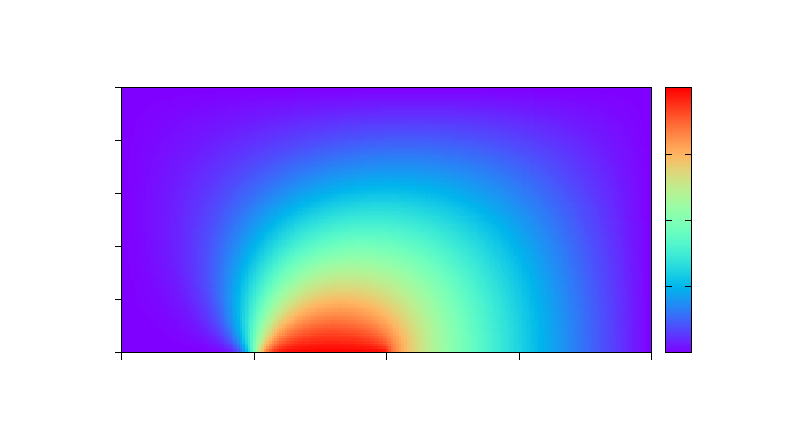
\includegraphics[width={368.50bp},height={198.40bp}]{smith_hutton_N201_Pe1.0e+01-inc}}%
    \gplfronttext
  \end{picture}%
\endgroup
\end{document}

	\caption{Numerical solution the the Smith--Hutton case for $\rho / \Gamma = 10$.}
	\label{fig:smith_hutton_N201_Pe1.0e+01}
	\vspace{1cm}
	% GNUPLOT: LaTeX picture with Postscript
\begingroup
  % Encoding inside the plot.  In the header of your document, this encoding
  % should to defined, e.g., by using
  % \usepackage[cp1252,<other encodings>]{inputenc}
  \inputencoding{cp1252}%
  \makeatletter
  \providecommand\color[2][]{%
    \GenericError{(gnuplot) \space\space\space\@spaces}{%
      Package color not loaded in conjunction with
      terminal option `colourtext'%
    }{See the gnuplot documentation for explanation.%
    }{Either use 'blacktext' in gnuplot or load the package
      color.sty in LaTeX.}%
    \renewcommand\color[2][]{}%
  }%
  \providecommand\includegraphics[2][]{%
    \GenericError{(gnuplot) \space\space\space\@spaces}{%
      Package graphicx or graphics not loaded%
    }{See the gnuplot documentation for explanation.%
    }{The gnuplot epslatex terminal needs graphicx.sty or graphics.sty.}%
    \renewcommand\includegraphics[2][]{}%
  }%
  \providecommand\rotatebox[2]{#2}%
  \@ifundefined{ifGPcolor}{%
    \newif\ifGPcolor
    \GPcolortrue
  }{}%
  \@ifundefined{ifGPblacktext}{%
    \newif\ifGPblacktext
    \GPblacktextfalse
  }{}%
  % define a \g@addto@macro without @ in the name:
  \let\gplgaddtomacro\g@addto@macro
  % define empty templates for all commands taking text:
  \gdef\gplbacktext{}%
  \gdef\gplfronttext{}%
  \makeatother
  \ifGPblacktext
    % no textcolor at all
    \def\colorrgb#1{}%
    \def\colorgray#1{}%
  \else
    % gray or color?
    \ifGPcolor
      \def\colorrgb#1{\color[rgb]{#1}}%
      \def\colorgray#1{\color[gray]{#1}}%
      \expandafter\def\csname LTw\endcsname{\color{white}}%
      \expandafter\def\csname LTb\endcsname{\color{black}}%
      \expandafter\def\csname LTa\endcsname{\color{black}}%
      \expandafter\def\csname LT0\endcsname{\color[rgb]{1,0,0}}%
      \expandafter\def\csname LT1\endcsname{\color[rgb]{0,1,0}}%
      \expandafter\def\csname LT2\endcsname{\color[rgb]{0,0,1}}%
      \expandafter\def\csname LT3\endcsname{\color[rgb]{1,0,1}}%
      \expandafter\def\csname LT4\endcsname{\color[rgb]{0,1,1}}%
      \expandafter\def\csname LT5\endcsname{\color[rgb]{1,1,0}}%
      \expandafter\def\csname LT6\endcsname{\color[rgb]{0,0,0}}%
      \expandafter\def\csname LT7\endcsname{\color[rgb]{1,0.3,0}}%
      \expandafter\def\csname LT8\endcsname{\color[rgb]{0.5,0.5,0.5}}%
    \else
      % gray
      \def\colorrgb#1{\color{black}}%
      \def\colorgray#1{\color[gray]{#1}}%
      \expandafter\def\csname LTw\endcsname{\color{white}}%
      \expandafter\def\csname LTb\endcsname{\color{black}}%
      \expandafter\def\csname LTa\endcsname{\color{black}}%
      \expandafter\def\csname LT0\endcsname{\color{black}}%
      \expandafter\def\csname LT1\endcsname{\color{black}}%
      \expandafter\def\csname LT2\endcsname{\color{black}}%
      \expandafter\def\csname LT3\endcsname{\color{black}}%
      \expandafter\def\csname LT4\endcsname{\color{black}}%
      \expandafter\def\csname LT5\endcsname{\color{black}}%
      \expandafter\def\csname LT6\endcsname{\color{black}}%
      \expandafter\def\csname LT7\endcsname{\color{black}}%
      \expandafter\def\csname LT8\endcsname{\color{black}}%
    \fi
  \fi
    \setlength{\unitlength}{0.0500bp}%
    \ifx\gptboxheight\undefined%
      \newlength{\gptboxheight}%
      \newlength{\gptboxwidth}%
      \newsavebox{\gptboxtext}%
    \fi%
    \setlength{\fboxrule}{0.5pt}%
    \setlength{\fboxsep}{1pt}%
    \definecolor{tbcol}{rgb}{1,1,1}%
\begin{picture}(7370.00,3968.00)%
    \gplgaddtomacro\gplbacktext{%
      \csname LTb\endcsname%%
      \put(814,719){\makebox(0,0)[r]{\strut{}0.0}}%
      \put(814,1234){\makebox(0,0)[r]{\strut{}0.2}}%
      \put(814,1748){\makebox(0,0)[r]{\strut{}0.4}}%
      \put(814,2263){\makebox(0,0)[r]{\strut{}0.6}}%
      \put(814,2777){\makebox(0,0)[r]{\strut{}0.8}}%
      \put(814,3292){\makebox(0,0)[r]{\strut{}1.0}}%
      \put(946,499){\makebox(0,0){\strut{}-1.0}}%
      \put(2233,499){\makebox(0,0){\strut{}-0.5}}%
      \put(3520,499){\makebox(0,0){\strut{}0.0}}%
      \put(4806,499){\makebox(0,0){\strut{}0.5}}%
      \put(6093,499){\makebox(0,0){\strut{}1.0}}%
    }%
    \gplgaddtomacro\gplfronttext{%
      \csname LTb\endcsname%%
      \put(209,2005){\rotatebox{-270}{\makebox(0,0){\strut{}$y \ (\mathrm{m})$}}}%
      \put(3519,169){\makebox(0,0){\strut{}$x \ (\mathrm{m})$}}%
      \csname LTb\endcsname%%
      \put(6611,719){\makebox(0,0)[l]{\strut{}0.0}}%
      \put(6611,1362){\makebox(0,0)[l]{\strut{}0.5}}%
      \put(6611,2005){\makebox(0,0)[l]{\strut{}1.0}}%
      \put(6611,2648){\makebox(0,0)[l]{\strut{}1.5}}%
      \put(6611,3292){\makebox(0,0)[l]{\strut{}2.0}}%
      \put(7073,2005){\rotatebox{-270}{\makebox(0,0){\strut{}$\phi$}}}%
      \put(3519,3622){\makebox(0,0){\strut{}\textbf{Smith--Hutton case} $(\mathrm{Pe} = 10^{2})$}}%
    }%
    \gplbacktext
    \put(0,0){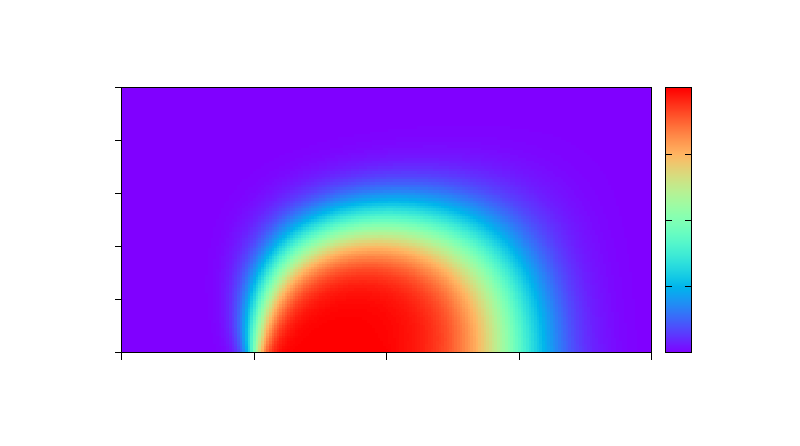
\includegraphics[width={368.50bp},height={198.40bp}]{figures/case_smith_hutton/smith_hutton_N201_Pe1.0e+02}}%
    \gplfronttext
  \end{picture}%
\endgroup

	\caption{Numerical solution the the Smith--Hutton case for $\rho / \Gamma = 10^2$.}
	\label{fig:smith_hutton_N201_Pe1.0e+02}
\end{figure}

% \begin{figure}[ht]
% 	\centering
% 	%	\fbox{% GNUPLOT: LaTeX picture with Postscript
\documentclass{minimal}
% Set font size
\makeatletter
\def\@ptsize{1}
\InputIfFileExists{size11.clo}{}{%
   \GenericError{(gnuplot) \space\space\space\@spaces}{%
      Gnuplot Error: File `size11.clo' not found! Could not set font size%
   }{See the gnuplot documentation for explanation.%
   }{For using a font size a file `size<fontsize>.clo' has to exist.
        Falling back ^^Jto default fontsize 10pt.}%
  \def\@ptsize{0}
  \input{size10.clo}%
}%
\makeatother
% Load packages
\usepackage{calc}
\usepackage{graphicx}
\usepackage{color}
\usepackage[cp1252]{inputenc}
\makeatletter
% Select an appropriate default driver (from TeXLive graphics.cfg)
\begingroup
  \chardef\x=0 %
  % check pdfTeX
  \@ifundefined{pdfoutput}{}{%
    \ifcase\pdfoutput
    \else
      \chardef\x=1 %
    \fi
  }%
  % check VTeX
  \@ifundefined{OpMode}{}{%
    \chardef\x=2 %
  }%
\expandafter\endgroup
\ifcase\x
  % default case
  \PassOptionsToPackage{dvips}{geometry}
\or
  % pdfTeX is running in pdf mode
  \PassOptionsToPackage{pdftex}{geometry}
\else
  % VTeX is running
  \PassOptionsToPackage{vtex}{geometry}
\fi
\makeatother
% Set papersize
\usepackage[papersize={368.50bp,198.40bp},text={368.50bp,198.40bp}]{geometry}
% No page numbers and no paragraph indentation
\pagestyle{empty}
\setlength{\parindent}{0bp}%
% Load configuration file
\InputIfFileExists{gnuplot.cfg}{%
  \typeout{Using configuration file gnuplot.cfg}%
}{%
 \typeout{No configuration file gnuplot.cfg found.}%
}%
%
\begin{document}
\begingroup
  % Encoding inside the plot.  In the header of your document, this encoding
  % should to defined, e.g., by using
  % \usepackage[cp1252,<other encodings>]{inputenc}
  \inputencoding{cp1252}%
  \makeatletter
  \providecommand\color[2][]{%
    \GenericError{(gnuplot) \space\space\space\@spaces}{%
      Package color not loaded in conjunction with
      terminal option `colourtext'%
    }{See the gnuplot documentation for explanation.%
    }{Either use 'blacktext' in gnuplot or load the package
      color.sty in LaTeX.}%
    \renewcommand\color[2][]{}%
  }%
  \providecommand\includegraphics[2][]{%
    \GenericError{(gnuplot) \space\space\space\@spaces}{%
      Package graphicx or graphics not loaded%
    }{See the gnuplot documentation for explanation.%
    }{The gnuplot epslatex terminal needs graphicx.sty or graphics.sty.}%
    \renewcommand\includegraphics[2][]{}%
  }%
  \providecommand\rotatebox[2]{#2}%
  \@ifundefined{ifGPcolor}{%
    \newif\ifGPcolor
    \GPcolortrue
  }{}%
  \@ifundefined{ifGPblacktext}{%
    \newif\ifGPblacktext
    \GPblacktextfalse
  }{}%
  % define a \g@addto@macro without @ in the name:
  \let\gplgaddtomacro\g@addto@macro
  % define empty templates for all commands taking text:
  \gdef\gplbacktext{}%
  \gdef\gplfronttext{}%
  \makeatother
  \ifGPblacktext
    % no textcolor at all
    \def\colorrgb#1{}%
    \def\colorgray#1{}%
  \else
    % gray or color?
    \ifGPcolor
      \def\colorrgb#1{\color[rgb]{#1}}%
      \def\colorgray#1{\color[gray]{#1}}%
      \expandafter\def\csname LTw\endcsname{\color{white}}%
      \expandafter\def\csname LTb\endcsname{\color{black}}%
      \expandafter\def\csname LTa\endcsname{\color{black}}%
      \expandafter\def\csname LT0\endcsname{\color[rgb]{1,0,0}}%
      \expandafter\def\csname LT1\endcsname{\color[rgb]{0,1,0}}%
      \expandafter\def\csname LT2\endcsname{\color[rgb]{0,0,1}}%
      \expandafter\def\csname LT3\endcsname{\color[rgb]{1,0,1}}%
      \expandafter\def\csname LT4\endcsname{\color[rgb]{0,1,1}}%
      \expandafter\def\csname LT5\endcsname{\color[rgb]{1,1,0}}%
      \expandafter\def\csname LT6\endcsname{\color[rgb]{0,0,0}}%
      \expandafter\def\csname LT7\endcsname{\color[rgb]{1,0.3,0}}%
      \expandafter\def\csname LT8\endcsname{\color[rgb]{0.5,0.5,0.5}}%
    \else
      % gray
      \def\colorrgb#1{\color{black}}%
      \def\colorgray#1{\color[gray]{#1}}%
      \expandafter\def\csname LTw\endcsname{\color{white}}%
      \expandafter\def\csname LTb\endcsname{\color{black}}%
      \expandafter\def\csname LTa\endcsname{\color{black}}%
      \expandafter\def\csname LT0\endcsname{\color{black}}%
      \expandafter\def\csname LT1\endcsname{\color{black}}%
      \expandafter\def\csname LT2\endcsname{\color{black}}%
      \expandafter\def\csname LT3\endcsname{\color{black}}%
      \expandafter\def\csname LT4\endcsname{\color{black}}%
      \expandafter\def\csname LT5\endcsname{\color{black}}%
      \expandafter\def\csname LT6\endcsname{\color{black}}%
      \expandafter\def\csname LT7\endcsname{\color{black}}%
      \expandafter\def\csname LT8\endcsname{\color{black}}%
    \fi
  \fi
    \setlength{\unitlength}{0.0500bp}%
    \ifx\gptboxheight\undefined%
      \newlength{\gptboxheight}%
      \newlength{\gptboxwidth}%
      \newsavebox{\gptboxtext}%
    \fi%
    \setlength{\fboxrule}{0.5pt}%
    \setlength{\fboxsep}{1pt}%
    \definecolor{tbcol}{rgb}{1,1,1}%
\begin{picture}(7370.00,3968.00)%
    \gplgaddtomacro\gplbacktext{%
      \csname LTb\endcsname%%
      \put(814,733){\makebox(0,0)[r]{\strut{}0.0}}%
      \put(814,1242){\makebox(0,0)[r]{\strut{}0.2}}%
      \put(814,1751){\makebox(0,0)[r]{\strut{}0.4}}%
      \put(814,2260){\makebox(0,0)[r]{\strut{}0.6}}%
      \put(814,2769){\makebox(0,0)[r]{\strut{}0.8}}%
      \put(814,3278){\makebox(0,0)[r]{\strut{}1.0}}%
      \put(1009,513){\makebox(0,0){\strut{}-1.0}}%
      \put(2282,513){\makebox(0,0){\strut{}-0.5}}%
      \put(3554,513){\makebox(0,0){\strut{}0.0}}%
      \put(4827,513){\makebox(0,0){\strut{}0.5}}%
      \put(6099,513){\makebox(0,0){\strut{}1.0}}%
    }%
    \gplgaddtomacro\gplfronttext{%
      \csname LTb\endcsname%%
      \put(209,2005){\rotatebox{-270}{\makebox(0,0){\strut{}$y \ (\mathrm{m})$}}}%
      \put(3554,183){\makebox(0,0){\strut{}$x \ (\mathrm{m})$}}%
      \csname LTb\endcsname%%
      \put(6612,733){\makebox(0,0)[l]{\strut{}0.0}}%
      \put(6612,1369){\makebox(0,0)[l]{\strut{}0.5}}%
      \put(6612,2005){\makebox(0,0)[l]{\strut{}1.0}}%
      \put(6612,2641){\makebox(0,0)[l]{\strut{}1.5}}%
      \put(6612,3278){\makebox(0,0)[l]{\strut{}2.0}}%
      \put(7074,2005){\rotatebox{-270}{\makebox(0,0){\strut{}$\phi$}}}%
      \put(3554,3608){\makebox(0,0){\strut{}\textbf{Smith--Hutton case} $(\rho / \Gamma = 10)$}}%
    }%
    \gplbacktext
    \put(0,0){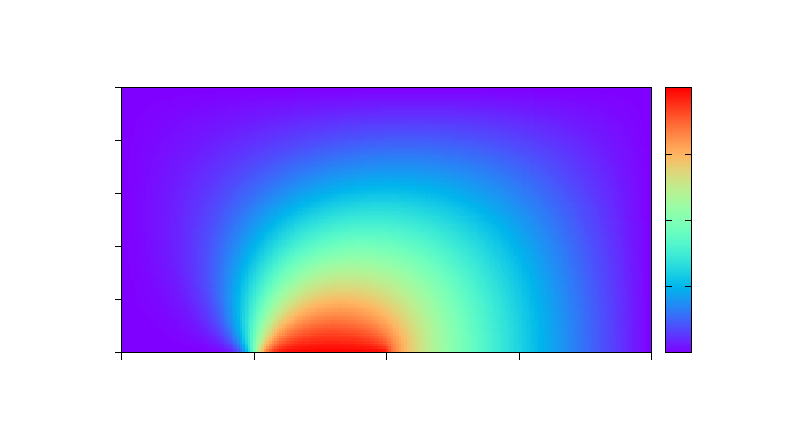
\includegraphics[width={368.50bp},height={198.40bp}]{smith_hutton_N201_Pe1.0e+01-inc}}%
    \gplfronttext
  \end{picture}%
\endgroup
\end{document}
}
% 	% GNUPLOT: LaTeX picture with Postscript
\documentclass{minimal}
% Set font size
\makeatletter
\def\@ptsize{1}
\InputIfFileExists{size11.clo}{}{%
   \GenericError{(gnuplot) \space\space\space\@spaces}{%
      Gnuplot Error: File `size11.clo' not found! Could not set font size%
   }{See the gnuplot documentation for explanation.%
   }{For using a font size a file `size<fontsize>.clo' has to exist.
        Falling back ^^Jto default fontsize 10pt.}%
  \def\@ptsize{0}
  \input{size10.clo}%
}%
\makeatother
% Load packages
\usepackage{calc}
\usepackage{graphicx}
\usepackage{color}
\usepackage[cp1252]{inputenc}
\makeatletter
% Select an appropriate default driver (from TeXLive graphics.cfg)
\begingroup
  \chardef\x=0 %
  % check pdfTeX
  \@ifundefined{pdfoutput}{}{%
    \ifcase\pdfoutput
    \else
      \chardef\x=1 %
    \fi
  }%
  % check VTeX
  \@ifundefined{OpMode}{}{%
    \chardef\x=2 %
  }%
\expandafter\endgroup
\ifcase\x
  % default case
  \PassOptionsToPackage{dvips}{geometry}
\or
  % pdfTeX is running in pdf mode
  \PassOptionsToPackage{pdftex}{geometry}
\else
  % VTeX is running
  \PassOptionsToPackage{vtex}{geometry}
\fi
\makeatother
% Set papersize
\usepackage[papersize={368.50bp,198.40bp},text={368.50bp,198.40bp}]{geometry}
% No page numbers and no paragraph indentation
\pagestyle{empty}
\setlength{\parindent}{0bp}%
% Load configuration file
\InputIfFileExists{gnuplot.cfg}{%
  \typeout{Using configuration file gnuplot.cfg}%
}{%
 \typeout{No configuration file gnuplot.cfg found.}%
}%
%
\begin{document}
\begingroup
  % Encoding inside the plot.  In the header of your document, this encoding
  % should to defined, e.g., by using
  % \usepackage[cp1252,<other encodings>]{inputenc}
  \inputencoding{cp1252}%
  \makeatletter
  \providecommand\color[2][]{%
    \GenericError{(gnuplot) \space\space\space\@spaces}{%
      Package color not loaded in conjunction with
      terminal option `colourtext'%
    }{See the gnuplot documentation for explanation.%
    }{Either use 'blacktext' in gnuplot or load the package
      color.sty in LaTeX.}%
    \renewcommand\color[2][]{}%
  }%
  \providecommand\includegraphics[2][]{%
    \GenericError{(gnuplot) \space\space\space\@spaces}{%
      Package graphicx or graphics not loaded%
    }{See the gnuplot documentation for explanation.%
    }{The gnuplot epslatex terminal needs graphicx.sty or graphics.sty.}%
    \renewcommand\includegraphics[2][]{}%
  }%
  \providecommand\rotatebox[2]{#2}%
  \@ifundefined{ifGPcolor}{%
    \newif\ifGPcolor
    \GPcolortrue
  }{}%
  \@ifundefined{ifGPblacktext}{%
    \newif\ifGPblacktext
    \GPblacktextfalse
  }{}%
  % define a \g@addto@macro without @ in the name:
  \let\gplgaddtomacro\g@addto@macro
  % define empty templates for all commands taking text:
  \gdef\gplbacktext{}%
  \gdef\gplfronttext{}%
  \makeatother
  \ifGPblacktext
    % no textcolor at all
    \def\colorrgb#1{}%
    \def\colorgray#1{}%
  \else
    % gray or color?
    \ifGPcolor
      \def\colorrgb#1{\color[rgb]{#1}}%
      \def\colorgray#1{\color[gray]{#1}}%
      \expandafter\def\csname LTw\endcsname{\color{white}}%
      \expandafter\def\csname LTb\endcsname{\color{black}}%
      \expandafter\def\csname LTa\endcsname{\color{black}}%
      \expandafter\def\csname LT0\endcsname{\color[rgb]{1,0,0}}%
      \expandafter\def\csname LT1\endcsname{\color[rgb]{0,1,0}}%
      \expandafter\def\csname LT2\endcsname{\color[rgb]{0,0,1}}%
      \expandafter\def\csname LT3\endcsname{\color[rgb]{1,0,1}}%
      \expandafter\def\csname LT4\endcsname{\color[rgb]{0,1,1}}%
      \expandafter\def\csname LT5\endcsname{\color[rgb]{1,1,0}}%
      \expandafter\def\csname LT6\endcsname{\color[rgb]{0,0,0}}%
      \expandafter\def\csname LT7\endcsname{\color[rgb]{1,0.3,0}}%
      \expandafter\def\csname LT8\endcsname{\color[rgb]{0.5,0.5,0.5}}%
    \else
      % gray
      \def\colorrgb#1{\color{black}}%
      \def\colorgray#1{\color[gray]{#1}}%
      \expandafter\def\csname LTw\endcsname{\color{white}}%
      \expandafter\def\csname LTb\endcsname{\color{black}}%
      \expandafter\def\csname LTa\endcsname{\color{black}}%
      \expandafter\def\csname LT0\endcsname{\color{black}}%
      \expandafter\def\csname LT1\endcsname{\color{black}}%
      \expandafter\def\csname LT2\endcsname{\color{black}}%
      \expandafter\def\csname LT3\endcsname{\color{black}}%
      \expandafter\def\csname LT4\endcsname{\color{black}}%
      \expandafter\def\csname LT5\endcsname{\color{black}}%
      \expandafter\def\csname LT6\endcsname{\color{black}}%
      \expandafter\def\csname LT7\endcsname{\color{black}}%
      \expandafter\def\csname LT8\endcsname{\color{black}}%
    \fi
  \fi
    \setlength{\unitlength}{0.0500bp}%
    \ifx\gptboxheight\undefined%
      \newlength{\gptboxheight}%
      \newlength{\gptboxwidth}%
      \newsavebox{\gptboxtext}%
    \fi%
    \setlength{\fboxrule}{0.5pt}%
    \setlength{\fboxsep}{1pt}%
    \definecolor{tbcol}{rgb}{1,1,1}%
\begin{picture}(7370.00,3968.00)%
    \gplgaddtomacro\gplbacktext{%
      \csname LTb\endcsname%%
      \put(814,733){\makebox(0,0)[r]{\strut{}0.0}}%
      \put(814,1242){\makebox(0,0)[r]{\strut{}0.2}}%
      \put(814,1751){\makebox(0,0)[r]{\strut{}0.4}}%
      \put(814,2260){\makebox(0,0)[r]{\strut{}0.6}}%
      \put(814,2769){\makebox(0,0)[r]{\strut{}0.8}}%
      \put(814,3278){\makebox(0,0)[r]{\strut{}1.0}}%
      \put(1009,513){\makebox(0,0){\strut{}-1.0}}%
      \put(2282,513){\makebox(0,0){\strut{}-0.5}}%
      \put(3554,513){\makebox(0,0){\strut{}0.0}}%
      \put(4827,513){\makebox(0,0){\strut{}0.5}}%
      \put(6099,513){\makebox(0,0){\strut{}1.0}}%
    }%
    \gplgaddtomacro\gplfronttext{%
      \csname LTb\endcsname%%
      \put(209,2005){\rotatebox{-270}{\makebox(0,0){\strut{}$y \ (\mathrm{m})$}}}%
      \put(3554,183){\makebox(0,0){\strut{}$x \ (\mathrm{m})$}}%
      \csname LTb\endcsname%%
      \put(6612,733){\makebox(0,0)[l]{\strut{}0.0}}%
      \put(6612,1369){\makebox(0,0)[l]{\strut{}0.5}}%
      \put(6612,2005){\makebox(0,0)[l]{\strut{}1.0}}%
      \put(6612,2641){\makebox(0,0)[l]{\strut{}1.5}}%
      \put(6612,3278){\makebox(0,0)[l]{\strut{}2.0}}%
      \put(7074,2005){\rotatebox{-270}{\makebox(0,0){\strut{}$\phi$}}}%
      \put(3554,3608){\makebox(0,0){\strut{}\textbf{Smith--Hutton case} $(\rho / \Gamma = 10)$}}%
    }%
    \gplbacktext
    \put(0,0){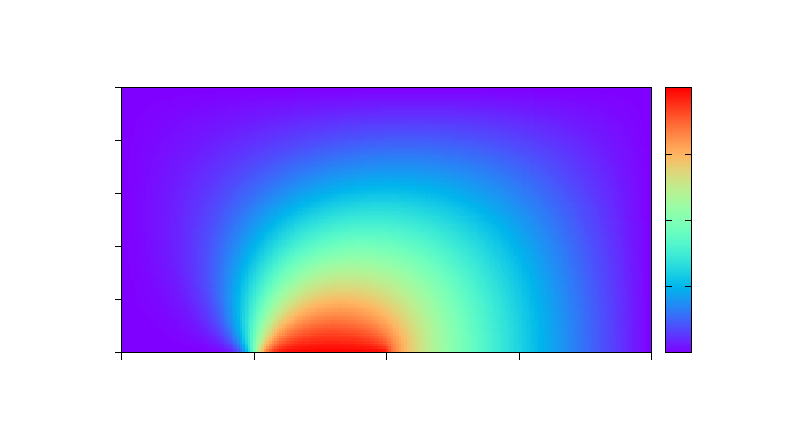
\includegraphics[width={368.50bp},height={198.40bp}]{smith_hutton_N201_Pe1.0e+01-inc}}%
    \gplfronttext
  \end{picture}%
\endgroup
\end{document}

% 	\caption{Numerical solution the the Smith--Hutton case for $\rho / \Gamma = 10$.}
% 	\label{fig:smith_hutton_N201_Pe1.0e+01}
% \end{figure}

% \begin{figure}[ht]
% 	\centering
% 	%	\fbox{% GNUPLOT: LaTeX picture with Postscript
\begingroup
  % Encoding inside the plot.  In the header of your document, this encoding
  % should to defined, e.g., by using
  % \usepackage[cp1252,<other encodings>]{inputenc}
  \inputencoding{cp1252}%
  \makeatletter
  \providecommand\color[2][]{%
    \GenericError{(gnuplot) \space\space\space\@spaces}{%
      Package color not loaded in conjunction with
      terminal option `colourtext'%
    }{See the gnuplot documentation for explanation.%
    }{Either use 'blacktext' in gnuplot or load the package
      color.sty in LaTeX.}%
    \renewcommand\color[2][]{}%
  }%
  \providecommand\includegraphics[2][]{%
    \GenericError{(gnuplot) \space\space\space\@spaces}{%
      Package graphicx or graphics not loaded%
    }{See the gnuplot documentation for explanation.%
    }{The gnuplot epslatex terminal needs graphicx.sty or graphics.sty.}%
    \renewcommand\includegraphics[2][]{}%
  }%
  \providecommand\rotatebox[2]{#2}%
  \@ifundefined{ifGPcolor}{%
    \newif\ifGPcolor
    \GPcolortrue
  }{}%
  \@ifundefined{ifGPblacktext}{%
    \newif\ifGPblacktext
    \GPblacktextfalse
  }{}%
  % define a \g@addto@macro without @ in the name:
  \let\gplgaddtomacro\g@addto@macro
  % define empty templates for all commands taking text:
  \gdef\gplbacktext{}%
  \gdef\gplfronttext{}%
  \makeatother
  \ifGPblacktext
    % no textcolor at all
    \def\colorrgb#1{}%
    \def\colorgray#1{}%
  \else
    % gray or color?
    \ifGPcolor
      \def\colorrgb#1{\color[rgb]{#1}}%
      \def\colorgray#1{\color[gray]{#1}}%
      \expandafter\def\csname LTw\endcsname{\color{white}}%
      \expandafter\def\csname LTb\endcsname{\color{black}}%
      \expandafter\def\csname LTa\endcsname{\color{black}}%
      \expandafter\def\csname LT0\endcsname{\color[rgb]{1,0,0}}%
      \expandafter\def\csname LT1\endcsname{\color[rgb]{0,1,0}}%
      \expandafter\def\csname LT2\endcsname{\color[rgb]{0,0,1}}%
      \expandafter\def\csname LT3\endcsname{\color[rgb]{1,0,1}}%
      \expandafter\def\csname LT4\endcsname{\color[rgb]{0,1,1}}%
      \expandafter\def\csname LT5\endcsname{\color[rgb]{1,1,0}}%
      \expandafter\def\csname LT6\endcsname{\color[rgb]{0,0,0}}%
      \expandafter\def\csname LT7\endcsname{\color[rgb]{1,0.3,0}}%
      \expandafter\def\csname LT8\endcsname{\color[rgb]{0.5,0.5,0.5}}%
    \else
      % gray
      \def\colorrgb#1{\color{black}}%
      \def\colorgray#1{\color[gray]{#1}}%
      \expandafter\def\csname LTw\endcsname{\color{white}}%
      \expandafter\def\csname LTb\endcsname{\color{black}}%
      \expandafter\def\csname LTa\endcsname{\color{black}}%
      \expandafter\def\csname LT0\endcsname{\color{black}}%
      \expandafter\def\csname LT1\endcsname{\color{black}}%
      \expandafter\def\csname LT2\endcsname{\color{black}}%
      \expandafter\def\csname LT3\endcsname{\color{black}}%
      \expandafter\def\csname LT4\endcsname{\color{black}}%
      \expandafter\def\csname LT5\endcsname{\color{black}}%
      \expandafter\def\csname LT6\endcsname{\color{black}}%
      \expandafter\def\csname LT7\endcsname{\color{black}}%
      \expandafter\def\csname LT8\endcsname{\color{black}}%
    \fi
  \fi
    \setlength{\unitlength}{0.0500bp}%
    \ifx\gptboxheight\undefined%
      \newlength{\gptboxheight}%
      \newlength{\gptboxwidth}%
      \newsavebox{\gptboxtext}%
    \fi%
    \setlength{\fboxrule}{0.5pt}%
    \setlength{\fboxsep}{1pt}%
    \definecolor{tbcol}{rgb}{1,1,1}%
\begin{picture}(7370.00,3968.00)%
    \gplgaddtomacro\gplbacktext{%
      \csname LTb\endcsname%%
      \put(814,719){\makebox(0,0)[r]{\strut{}0.0}}%
      \put(814,1234){\makebox(0,0)[r]{\strut{}0.2}}%
      \put(814,1748){\makebox(0,0)[r]{\strut{}0.4}}%
      \put(814,2263){\makebox(0,0)[r]{\strut{}0.6}}%
      \put(814,2777){\makebox(0,0)[r]{\strut{}0.8}}%
      \put(814,3292){\makebox(0,0)[r]{\strut{}1.0}}%
      \put(946,499){\makebox(0,0){\strut{}-1.0}}%
      \put(2233,499){\makebox(0,0){\strut{}-0.5}}%
      \put(3520,499){\makebox(0,0){\strut{}0.0}}%
      \put(4806,499){\makebox(0,0){\strut{}0.5}}%
      \put(6093,499){\makebox(0,0){\strut{}1.0}}%
    }%
    \gplgaddtomacro\gplfronttext{%
      \csname LTb\endcsname%%
      \put(209,2005){\rotatebox{-270}{\makebox(0,0){\strut{}$y \ (\mathrm{m})$}}}%
      \put(3519,169){\makebox(0,0){\strut{}$x \ (\mathrm{m})$}}%
      \csname LTb\endcsname%%
      \put(6611,719){\makebox(0,0)[l]{\strut{}0.0}}%
      \put(6611,1362){\makebox(0,0)[l]{\strut{}0.5}}%
      \put(6611,2005){\makebox(0,0)[l]{\strut{}1.0}}%
      \put(6611,2648){\makebox(0,0)[l]{\strut{}1.5}}%
      \put(6611,3292){\makebox(0,0)[l]{\strut{}2.0}}%
      \put(7073,2005){\rotatebox{-270}{\makebox(0,0){\strut{}$\phi$}}}%
      \put(3519,3622){\makebox(0,0){\strut{}\textbf{Smith--Hutton case} $(\mathrm{Pe} = 10^{2})$}}%
    }%
    \gplbacktext
    \put(0,0){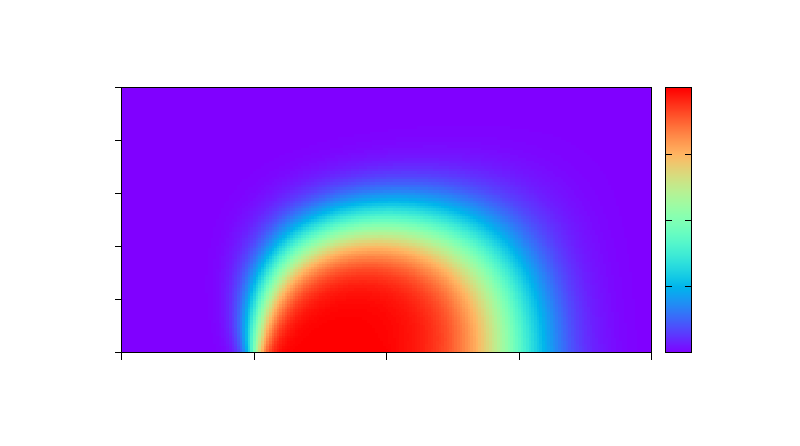
\includegraphics[width={368.50bp},height={198.40bp}]{figures/case_smith_hutton/smith_hutton_N201_Pe1.0e+02}}%
    \gplfronttext
  \end{picture}%
\endgroup
}
% 	% GNUPLOT: LaTeX picture with Postscript
\begingroup
  % Encoding inside the plot.  In the header of your document, this encoding
  % should to defined, e.g., by using
  % \usepackage[cp1252,<other encodings>]{inputenc}
  \inputencoding{cp1252}%
  \makeatletter
  \providecommand\color[2][]{%
    \GenericError{(gnuplot) \space\space\space\@spaces}{%
      Package color not loaded in conjunction with
      terminal option `colourtext'%
    }{See the gnuplot documentation for explanation.%
    }{Either use 'blacktext' in gnuplot or load the package
      color.sty in LaTeX.}%
    \renewcommand\color[2][]{}%
  }%
  \providecommand\includegraphics[2][]{%
    \GenericError{(gnuplot) \space\space\space\@spaces}{%
      Package graphicx or graphics not loaded%
    }{See the gnuplot documentation for explanation.%
    }{The gnuplot epslatex terminal needs graphicx.sty or graphics.sty.}%
    \renewcommand\includegraphics[2][]{}%
  }%
  \providecommand\rotatebox[2]{#2}%
  \@ifundefined{ifGPcolor}{%
    \newif\ifGPcolor
    \GPcolortrue
  }{}%
  \@ifundefined{ifGPblacktext}{%
    \newif\ifGPblacktext
    \GPblacktextfalse
  }{}%
  % define a \g@addto@macro without @ in the name:
  \let\gplgaddtomacro\g@addto@macro
  % define empty templates for all commands taking text:
  \gdef\gplbacktext{}%
  \gdef\gplfronttext{}%
  \makeatother
  \ifGPblacktext
    % no textcolor at all
    \def\colorrgb#1{}%
    \def\colorgray#1{}%
  \else
    % gray or color?
    \ifGPcolor
      \def\colorrgb#1{\color[rgb]{#1}}%
      \def\colorgray#1{\color[gray]{#1}}%
      \expandafter\def\csname LTw\endcsname{\color{white}}%
      \expandafter\def\csname LTb\endcsname{\color{black}}%
      \expandafter\def\csname LTa\endcsname{\color{black}}%
      \expandafter\def\csname LT0\endcsname{\color[rgb]{1,0,0}}%
      \expandafter\def\csname LT1\endcsname{\color[rgb]{0,1,0}}%
      \expandafter\def\csname LT2\endcsname{\color[rgb]{0,0,1}}%
      \expandafter\def\csname LT3\endcsname{\color[rgb]{1,0,1}}%
      \expandafter\def\csname LT4\endcsname{\color[rgb]{0,1,1}}%
      \expandafter\def\csname LT5\endcsname{\color[rgb]{1,1,0}}%
      \expandafter\def\csname LT6\endcsname{\color[rgb]{0,0,0}}%
      \expandafter\def\csname LT7\endcsname{\color[rgb]{1,0.3,0}}%
      \expandafter\def\csname LT8\endcsname{\color[rgb]{0.5,0.5,0.5}}%
    \else
      % gray
      \def\colorrgb#1{\color{black}}%
      \def\colorgray#1{\color[gray]{#1}}%
      \expandafter\def\csname LTw\endcsname{\color{white}}%
      \expandafter\def\csname LTb\endcsname{\color{black}}%
      \expandafter\def\csname LTa\endcsname{\color{black}}%
      \expandafter\def\csname LT0\endcsname{\color{black}}%
      \expandafter\def\csname LT1\endcsname{\color{black}}%
      \expandafter\def\csname LT2\endcsname{\color{black}}%
      \expandafter\def\csname LT3\endcsname{\color{black}}%
      \expandafter\def\csname LT4\endcsname{\color{black}}%
      \expandafter\def\csname LT5\endcsname{\color{black}}%
      \expandafter\def\csname LT6\endcsname{\color{black}}%
      \expandafter\def\csname LT7\endcsname{\color{black}}%
      \expandafter\def\csname LT8\endcsname{\color{black}}%
    \fi
  \fi
    \setlength{\unitlength}{0.0500bp}%
    \ifx\gptboxheight\undefined%
      \newlength{\gptboxheight}%
      \newlength{\gptboxwidth}%
      \newsavebox{\gptboxtext}%
    \fi%
    \setlength{\fboxrule}{0.5pt}%
    \setlength{\fboxsep}{1pt}%
    \definecolor{tbcol}{rgb}{1,1,1}%
\begin{picture}(7370.00,3968.00)%
    \gplgaddtomacro\gplbacktext{%
      \csname LTb\endcsname%%
      \put(814,719){\makebox(0,0)[r]{\strut{}0.0}}%
      \put(814,1234){\makebox(0,0)[r]{\strut{}0.2}}%
      \put(814,1748){\makebox(0,0)[r]{\strut{}0.4}}%
      \put(814,2263){\makebox(0,0)[r]{\strut{}0.6}}%
      \put(814,2777){\makebox(0,0)[r]{\strut{}0.8}}%
      \put(814,3292){\makebox(0,0)[r]{\strut{}1.0}}%
      \put(946,499){\makebox(0,0){\strut{}-1.0}}%
      \put(2233,499){\makebox(0,0){\strut{}-0.5}}%
      \put(3520,499){\makebox(0,0){\strut{}0.0}}%
      \put(4806,499){\makebox(0,0){\strut{}0.5}}%
      \put(6093,499){\makebox(0,0){\strut{}1.0}}%
    }%
    \gplgaddtomacro\gplfronttext{%
      \csname LTb\endcsname%%
      \put(209,2005){\rotatebox{-270}{\makebox(0,0){\strut{}$y \ (\mathrm{m})$}}}%
      \put(3519,169){\makebox(0,0){\strut{}$x \ (\mathrm{m})$}}%
      \csname LTb\endcsname%%
      \put(6611,719){\makebox(0,0)[l]{\strut{}0.0}}%
      \put(6611,1362){\makebox(0,0)[l]{\strut{}0.5}}%
      \put(6611,2005){\makebox(0,0)[l]{\strut{}1.0}}%
      \put(6611,2648){\makebox(0,0)[l]{\strut{}1.5}}%
      \put(6611,3292){\makebox(0,0)[l]{\strut{}2.0}}%
      \put(7073,2005){\rotatebox{-270}{\makebox(0,0){\strut{}$\phi$}}}%
      \put(3519,3622){\makebox(0,0){\strut{}\textbf{Smith--Hutton case} $(\mathrm{Pe} = 10^{2})$}}%
    }%
    \gplbacktext
    \put(0,0){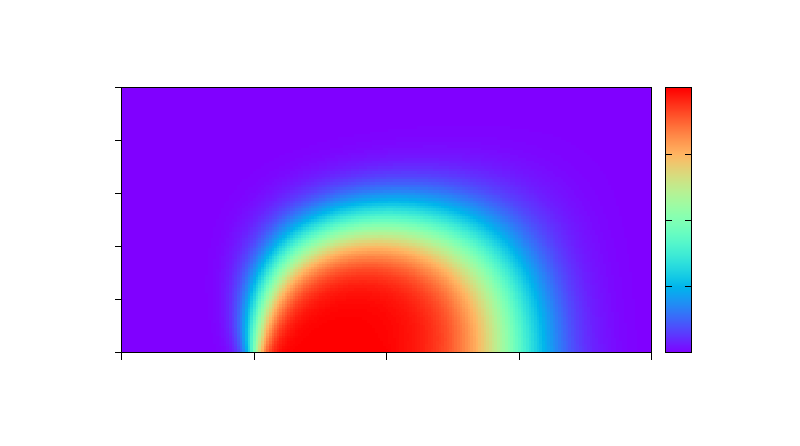
\includegraphics[width={368.50bp},height={198.40bp}]{figures/case_smith_hutton/smith_hutton_N201_Pe1.0e+02}}%
    \gplfronttext
  \end{picture}%
\endgroup

% 	\caption{Numerical solution the the Smith--Hutton case for $\rho / \Gamma = 10^2$.}
% 	\label{fig:smith_hutton_N201_Pe1.0e+02}
% \end{figure}


\clearpage
Figures \ref{fig:smith_hutton_N201_Pe1.0e+04} and
\ref{fig:smith_hutton_N201_Pe1.0e+09} show the numerical solution to the
Smith--Hutton case for $\rho / \Gamma = 10^4$ and $10^9$ respectively. There is
no apparent difference between two solution, what induces to think that for
$\rho / \Gamma > 10^4$ the solution stays approximately the same. There are
apparent discrepancies between the cases $\rho / \Gamma = 10^2$ and $\rho /
\Gamma = 10^4$. In the latter transport clearly takes over diffusion, as the
several color bands have approximately the same width, meaning diffusion has
much less strength than transport. 

\begin{figure}[ht]
	\centering
	% GNUPLOT: LaTeX picture with Postscript
\begingroup
  % Encoding inside the plot.  In the header of your document, this encoding
  % should to defined, e.g., by using
  % \usepackage[cp1252,<other encodings>]{inputenc}
  \inputencoding{cp1252}%
  \makeatletter
  \providecommand\color[2][]{%
    \GenericError{(gnuplot) \space\space\space\@spaces}{%
      Package color not loaded in conjunction with
      terminal option `colourtext'%
    }{See the gnuplot documentation for explanation.%
    }{Either use 'blacktext' in gnuplot or load the package
      color.sty in LaTeX.}%
    \renewcommand\color[2][]{}%
  }%
  \providecommand\includegraphics[2][]{%
    \GenericError{(gnuplot) \space\space\space\@spaces}{%
      Package graphicx or graphics not loaded%
    }{See the gnuplot documentation for explanation.%
    }{The gnuplot epslatex terminal needs graphicx.sty or graphics.sty.}%
    \renewcommand\includegraphics[2][]{}%
  }%
  \providecommand\rotatebox[2]{#2}%
  \@ifundefined{ifGPcolor}{%
    \newif\ifGPcolor
    \GPcolortrue
  }{}%
  \@ifundefined{ifGPblacktext}{%
    \newif\ifGPblacktext
    \GPblacktextfalse
  }{}%
  % define a \g@addto@macro without @ in the name:
  \let\gplgaddtomacro\g@addto@macro
  % define empty templates for all commands taking text:
  \gdef\gplbacktext{}%
  \gdef\gplfronttext{}%
  \makeatother
  \ifGPblacktext
    % no textcolor at all
    \def\colorrgb#1{}%
    \def\colorgray#1{}%
  \else
    % gray or color?
    \ifGPcolor
      \def\colorrgb#1{\color[rgb]{#1}}%
      \def\colorgray#1{\color[gray]{#1}}%
      \expandafter\def\csname LTw\endcsname{\color{white}}%
      \expandafter\def\csname LTb\endcsname{\color{black}}%
      \expandafter\def\csname LTa\endcsname{\color{black}}%
      \expandafter\def\csname LT0\endcsname{\color[rgb]{1,0,0}}%
      \expandafter\def\csname LT1\endcsname{\color[rgb]{0,1,0}}%
      \expandafter\def\csname LT2\endcsname{\color[rgb]{0,0,1}}%
      \expandafter\def\csname LT3\endcsname{\color[rgb]{1,0,1}}%
      \expandafter\def\csname LT4\endcsname{\color[rgb]{0,1,1}}%
      \expandafter\def\csname LT5\endcsname{\color[rgb]{1,1,0}}%
      \expandafter\def\csname LT6\endcsname{\color[rgb]{0,0,0}}%
      \expandafter\def\csname LT7\endcsname{\color[rgb]{1,0.3,0}}%
      \expandafter\def\csname LT8\endcsname{\color[rgb]{0.5,0.5,0.5}}%
    \else
      % gray
      \def\colorrgb#1{\color{black}}%
      \def\colorgray#1{\color[gray]{#1}}%
      \expandafter\def\csname LTw\endcsname{\color{white}}%
      \expandafter\def\csname LTb\endcsname{\color{black}}%
      \expandafter\def\csname LTa\endcsname{\color{black}}%
      \expandafter\def\csname LT0\endcsname{\color{black}}%
      \expandafter\def\csname LT1\endcsname{\color{black}}%
      \expandafter\def\csname LT2\endcsname{\color{black}}%
      \expandafter\def\csname LT3\endcsname{\color{black}}%
      \expandafter\def\csname LT4\endcsname{\color{black}}%
      \expandafter\def\csname LT5\endcsname{\color{black}}%
      \expandafter\def\csname LT6\endcsname{\color{black}}%
      \expandafter\def\csname LT7\endcsname{\color{black}}%
      \expandafter\def\csname LT8\endcsname{\color{black}}%
    \fi
  \fi
    \setlength{\unitlength}{0.0500bp}%
    \ifx\gptboxheight\undefined%
      \newlength{\gptboxheight}%
      \newlength{\gptboxwidth}%
      \newsavebox{\gptboxtext}%
    \fi%
    \setlength{\fboxrule}{0.5pt}%
    \setlength{\fboxsep}{1pt}%
    \definecolor{tbcol}{rgb}{1,1,1}%
\begin{picture}(7370.00,3968.00)%
    \gplgaddtomacro\gplbacktext{%
      \csname LTb\endcsname%%
      \put(814,719){\makebox(0,0)[r]{\strut{}0.0}}%
      \put(814,1234){\makebox(0,0)[r]{\strut{}0.2}}%
      \put(814,1748){\makebox(0,0)[r]{\strut{}0.4}}%
      \put(814,2263){\makebox(0,0)[r]{\strut{}0.6}}%
      \put(814,2777){\makebox(0,0)[r]{\strut{}0.8}}%
      \put(814,3292){\makebox(0,0)[r]{\strut{}1.0}}%
      \put(946,499){\makebox(0,0){\strut{}-1.0}}%
      \put(2233,499){\makebox(0,0){\strut{}-0.5}}%
      \put(3520,499){\makebox(0,0){\strut{}0.0}}%
      \put(4806,499){\makebox(0,0){\strut{}0.5}}%
      \put(6093,499){\makebox(0,0){\strut{}1.0}}%
    }%
    \gplgaddtomacro\gplfronttext{%
      \csname LTb\endcsname%%
      \put(209,2005){\rotatebox{-270}{\makebox(0,0){\strut{}$y \ (\mathrm{m})$}}}%
      \put(3519,169){\makebox(0,0){\strut{}$x \ (\mathrm{m})$}}%
      \csname LTb\endcsname%%
      \put(6611,719){\makebox(0,0)[l]{\strut{}0.0}}%
      \put(6611,1362){\makebox(0,0)[l]{\strut{}0.5}}%
      \put(6611,2005){\makebox(0,0)[l]{\strut{}1.0}}%
      \put(6611,2648){\makebox(0,0)[l]{\strut{}1.5}}%
      \put(6611,3292){\makebox(0,0)[l]{\strut{}2.0}}%
      \put(7073,2005){\rotatebox{-270}{\makebox(0,0){\strut{}$\phi$}}}%
      \put(3519,3622){\makebox(0,0){\strut{}\textbf{Smith--Hutton case} $(\mathrm{Pe} = 10^{4})$}}%
    }%
    \gplbacktext
    \put(0,0){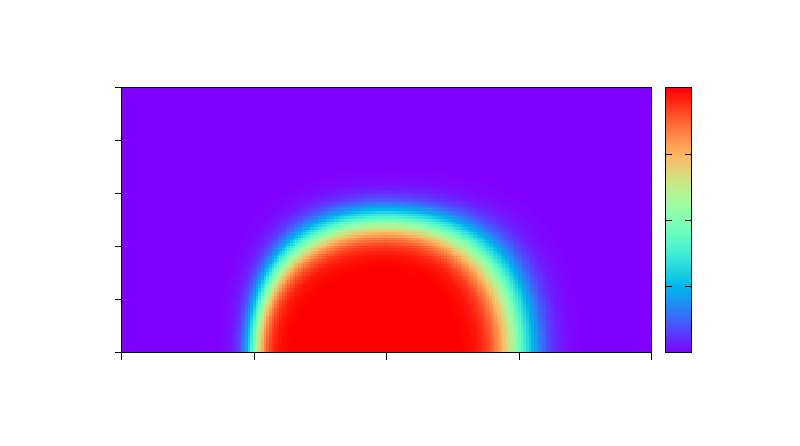
\includegraphics[width={368.50bp},height={198.40bp}]{figures/case_smith_hutton/smith_hutton_N201_Pe1.0e+04}}%
    \gplfronttext
  \end{picture}%
\endgroup

	\caption{Numerical solution the the Smith--Hutton case for $\rho / \Gamma = 10^4$.}
	\label{fig:smith_hutton_N201_Pe1.0e+04}
	\vspace{1cm}
	% GNUPLOT: LaTeX picture with Postscript
\begingroup
  % Encoding inside the plot.  In the header of your document, this encoding
  % should to defined, e.g., by using
  % \usepackage[cp1252,<other encodings>]{inputenc}
  \inputencoding{cp1252}%
  \makeatletter
  \providecommand\color[2][]{%
    \GenericError{(gnuplot) \space\space\space\@spaces}{%
      Package color not loaded in conjunction with
      terminal option `colourtext'%
    }{See the gnuplot documentation for explanation.%
    }{Either use 'blacktext' in gnuplot or load the package
      color.sty in LaTeX.}%
    \renewcommand\color[2][]{}%
  }%
  \providecommand\includegraphics[2][]{%
    \GenericError{(gnuplot) \space\space\space\@spaces}{%
      Package graphicx or graphics not loaded%
    }{See the gnuplot documentation for explanation.%
    }{The gnuplot epslatex terminal needs graphicx.sty or graphics.sty.}%
    \renewcommand\includegraphics[2][]{}%
  }%
  \providecommand\rotatebox[2]{#2}%
  \@ifundefined{ifGPcolor}{%
    \newif\ifGPcolor
    \GPcolortrue
  }{}%
  \@ifundefined{ifGPblacktext}{%
    \newif\ifGPblacktext
    \GPblacktextfalse
  }{}%
  % define a \g@addto@macro without @ in the name:
  \let\gplgaddtomacro\g@addto@macro
  % define empty templates for all commands taking text:
  \gdef\gplbacktext{}%
  \gdef\gplfronttext{}%
  \makeatother
  \ifGPblacktext
    % no textcolor at all
    \def\colorrgb#1{}%
    \def\colorgray#1{}%
  \else
    % gray or color?
    \ifGPcolor
      \def\colorrgb#1{\color[rgb]{#1}}%
      \def\colorgray#1{\color[gray]{#1}}%
      \expandafter\def\csname LTw\endcsname{\color{white}}%
      \expandafter\def\csname LTb\endcsname{\color{black}}%
      \expandafter\def\csname LTa\endcsname{\color{black}}%
      \expandafter\def\csname LT0\endcsname{\color[rgb]{1,0,0}}%
      \expandafter\def\csname LT1\endcsname{\color[rgb]{0,1,0}}%
      \expandafter\def\csname LT2\endcsname{\color[rgb]{0,0,1}}%
      \expandafter\def\csname LT3\endcsname{\color[rgb]{1,0,1}}%
      \expandafter\def\csname LT4\endcsname{\color[rgb]{0,1,1}}%
      \expandafter\def\csname LT5\endcsname{\color[rgb]{1,1,0}}%
      \expandafter\def\csname LT6\endcsname{\color[rgb]{0,0,0}}%
      \expandafter\def\csname LT7\endcsname{\color[rgb]{1,0.3,0}}%
      \expandafter\def\csname LT8\endcsname{\color[rgb]{0.5,0.5,0.5}}%
    \else
      % gray
      \def\colorrgb#1{\color{black}}%
      \def\colorgray#1{\color[gray]{#1}}%
      \expandafter\def\csname LTw\endcsname{\color{white}}%
      \expandafter\def\csname LTb\endcsname{\color{black}}%
      \expandafter\def\csname LTa\endcsname{\color{black}}%
      \expandafter\def\csname LT0\endcsname{\color{black}}%
      \expandafter\def\csname LT1\endcsname{\color{black}}%
      \expandafter\def\csname LT2\endcsname{\color{black}}%
      \expandafter\def\csname LT3\endcsname{\color{black}}%
      \expandafter\def\csname LT4\endcsname{\color{black}}%
      \expandafter\def\csname LT5\endcsname{\color{black}}%
      \expandafter\def\csname LT6\endcsname{\color{black}}%
      \expandafter\def\csname LT7\endcsname{\color{black}}%
      \expandafter\def\csname LT8\endcsname{\color{black}}%
    \fi
  \fi
    \setlength{\unitlength}{0.0500bp}%
    \ifx\gptboxheight\undefined%
      \newlength{\gptboxheight}%
      \newlength{\gptboxwidth}%
      \newsavebox{\gptboxtext}%
    \fi%
    \setlength{\fboxrule}{0.5pt}%
    \setlength{\fboxsep}{1pt}%
    \definecolor{tbcol}{rgb}{1,1,1}%
\begin{picture}(7370.00,3968.00)%
    \gplgaddtomacro\gplbacktext{%
      \csname LTb\endcsname%%
      \put(814,733){\makebox(0,0)[r]{\strut{}$0$}}%
      \put(814,1242){\makebox(0,0)[r]{\strut{}$0.2$}}%
      \put(814,1751){\makebox(0,0)[r]{\strut{}$0.4$}}%
      \put(814,2260){\makebox(0,0)[r]{\strut{}$0.6$}}%
      \put(814,2769){\makebox(0,0)[r]{\strut{}$0.8$}}%
      \put(814,3278){\makebox(0,0)[r]{\strut{}$1$}}%
      \put(1009,513){\makebox(0,0){\strut{}-1.0}}%
      \put(2282,513){\makebox(0,0){\strut{}-0.5}}%
      \put(3554,513){\makebox(0,0){\strut{}0.0}}%
      \put(4827,513){\makebox(0,0){\strut{}0.5}}%
      \put(6099,513){\makebox(0,0){\strut{}1.0}}%
    }%
    \gplgaddtomacro\gplfronttext{%
      \csname LTb\endcsname%%
      \put(209,2005){\rotatebox{-270}{\makebox(0,0){\strut{}$y \ (\mathrm{m})$}}}%
      \put(3554,183){\makebox(0,0){\strut{}$x \ (\mathrm{m})$}}%
      \csname LTb\endcsname%%
      \put(6612,733){\makebox(0,0)[l]{\strut{}0.0}}%
      \put(6612,1369){\makebox(0,0)[l]{\strut{}0.5}}%
      \put(6612,2005){\makebox(0,0)[l]{\strut{}1.0}}%
      \put(6612,2641){\makebox(0,0)[l]{\strut{}1.5}}%
      \put(6612,3278){\makebox(0,0)[l]{\strut{}2.0}}%
      \put(7074,2005){\rotatebox{-270}{\makebox(0,0){\strut{}$\phi$}}}%
      \put(3554,3608){\makebox(0,0){\strut{}\textbf{Smith--Hutton case} $(\rho / \Gamma = 10^{9})$}}%
    }%
    \gplbacktext
    \put(0,0){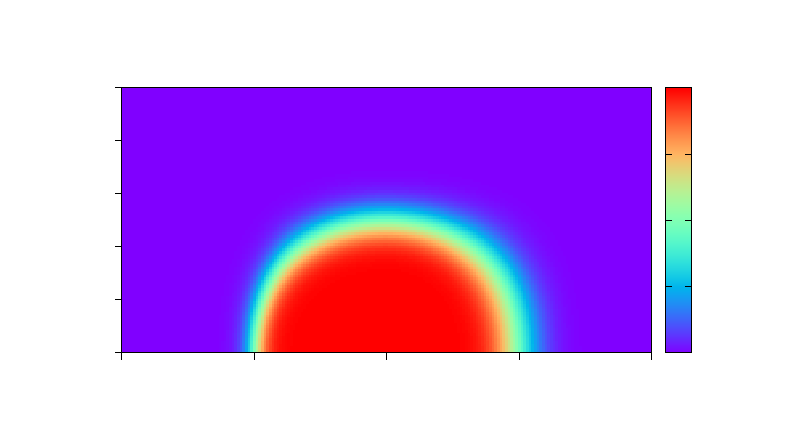
\includegraphics[width={368.50bp},height={198.40bp}]{figures/case_smith_hutton/smith_hutton_N201_Pe1.0e+09}}%
    \gplfronttext
  \end{picture}%
\endgroup

	\caption{Numerical solution the the Smith--Hutton case for $\rho / \Gamma = 10^9$.}
	\label{fig:smith_hutton_N201_Pe1.0e+09}
\end{figure}


% \begin{figure}[ht]
% 	\centering
% 	%	\fbox{% GNUPLOT: LaTeX picture with Postscript
\begingroup
  % Encoding inside the plot.  In the header of your document, this encoding
  % should to defined, e.g., by using
  % \usepackage[cp1252,<other encodings>]{inputenc}
  \inputencoding{cp1252}%
  \makeatletter
  \providecommand\color[2][]{%
    \GenericError{(gnuplot) \space\space\space\@spaces}{%
      Package color not loaded in conjunction with
      terminal option `colourtext'%
    }{See the gnuplot documentation for explanation.%
    }{Either use 'blacktext' in gnuplot or load the package
      color.sty in LaTeX.}%
    \renewcommand\color[2][]{}%
  }%
  \providecommand\includegraphics[2][]{%
    \GenericError{(gnuplot) \space\space\space\@spaces}{%
      Package graphicx or graphics not loaded%
    }{See the gnuplot documentation for explanation.%
    }{The gnuplot epslatex terminal needs graphicx.sty or graphics.sty.}%
    \renewcommand\includegraphics[2][]{}%
  }%
  \providecommand\rotatebox[2]{#2}%
  \@ifundefined{ifGPcolor}{%
    \newif\ifGPcolor
    \GPcolortrue
  }{}%
  \@ifundefined{ifGPblacktext}{%
    \newif\ifGPblacktext
    \GPblacktextfalse
  }{}%
  % define a \g@addto@macro without @ in the name:
  \let\gplgaddtomacro\g@addto@macro
  % define empty templates for all commands taking text:
  \gdef\gplbacktext{}%
  \gdef\gplfronttext{}%
  \makeatother
  \ifGPblacktext
    % no textcolor at all
    \def\colorrgb#1{}%
    \def\colorgray#1{}%
  \else
    % gray or color?
    \ifGPcolor
      \def\colorrgb#1{\color[rgb]{#1}}%
      \def\colorgray#1{\color[gray]{#1}}%
      \expandafter\def\csname LTw\endcsname{\color{white}}%
      \expandafter\def\csname LTb\endcsname{\color{black}}%
      \expandafter\def\csname LTa\endcsname{\color{black}}%
      \expandafter\def\csname LT0\endcsname{\color[rgb]{1,0,0}}%
      \expandafter\def\csname LT1\endcsname{\color[rgb]{0,1,0}}%
      \expandafter\def\csname LT2\endcsname{\color[rgb]{0,0,1}}%
      \expandafter\def\csname LT3\endcsname{\color[rgb]{1,0,1}}%
      \expandafter\def\csname LT4\endcsname{\color[rgb]{0,1,1}}%
      \expandafter\def\csname LT5\endcsname{\color[rgb]{1,1,0}}%
      \expandafter\def\csname LT6\endcsname{\color[rgb]{0,0,0}}%
      \expandafter\def\csname LT7\endcsname{\color[rgb]{1,0.3,0}}%
      \expandafter\def\csname LT8\endcsname{\color[rgb]{0.5,0.5,0.5}}%
    \else
      % gray
      \def\colorrgb#1{\color{black}}%
      \def\colorgray#1{\color[gray]{#1}}%
      \expandafter\def\csname LTw\endcsname{\color{white}}%
      \expandafter\def\csname LTb\endcsname{\color{black}}%
      \expandafter\def\csname LTa\endcsname{\color{black}}%
      \expandafter\def\csname LT0\endcsname{\color{black}}%
      \expandafter\def\csname LT1\endcsname{\color{black}}%
      \expandafter\def\csname LT2\endcsname{\color{black}}%
      \expandafter\def\csname LT3\endcsname{\color{black}}%
      \expandafter\def\csname LT4\endcsname{\color{black}}%
      \expandafter\def\csname LT5\endcsname{\color{black}}%
      \expandafter\def\csname LT6\endcsname{\color{black}}%
      \expandafter\def\csname LT7\endcsname{\color{black}}%
      \expandafter\def\csname LT8\endcsname{\color{black}}%
    \fi
  \fi
    \setlength{\unitlength}{0.0500bp}%
    \ifx\gptboxheight\undefined%
      \newlength{\gptboxheight}%
      \newlength{\gptboxwidth}%
      \newsavebox{\gptboxtext}%
    \fi%
    \setlength{\fboxrule}{0.5pt}%
    \setlength{\fboxsep}{1pt}%
    \definecolor{tbcol}{rgb}{1,1,1}%
\begin{picture}(7370.00,3968.00)%
    \gplgaddtomacro\gplbacktext{%
      \csname LTb\endcsname%%
      \put(814,719){\makebox(0,0)[r]{\strut{}0.0}}%
      \put(814,1234){\makebox(0,0)[r]{\strut{}0.2}}%
      \put(814,1748){\makebox(0,0)[r]{\strut{}0.4}}%
      \put(814,2263){\makebox(0,0)[r]{\strut{}0.6}}%
      \put(814,2777){\makebox(0,0)[r]{\strut{}0.8}}%
      \put(814,3292){\makebox(0,0)[r]{\strut{}1.0}}%
      \put(946,499){\makebox(0,0){\strut{}-1.0}}%
      \put(2233,499){\makebox(0,0){\strut{}-0.5}}%
      \put(3520,499){\makebox(0,0){\strut{}0.0}}%
      \put(4806,499){\makebox(0,0){\strut{}0.5}}%
      \put(6093,499){\makebox(0,0){\strut{}1.0}}%
    }%
    \gplgaddtomacro\gplfronttext{%
      \csname LTb\endcsname%%
      \put(209,2005){\rotatebox{-270}{\makebox(0,0){\strut{}$y \ (\mathrm{m})$}}}%
      \put(3519,169){\makebox(0,0){\strut{}$x \ (\mathrm{m})$}}%
      \csname LTb\endcsname%%
      \put(6611,719){\makebox(0,0)[l]{\strut{}0.0}}%
      \put(6611,1362){\makebox(0,0)[l]{\strut{}0.5}}%
      \put(6611,2005){\makebox(0,0)[l]{\strut{}1.0}}%
      \put(6611,2648){\makebox(0,0)[l]{\strut{}1.5}}%
      \put(6611,3292){\makebox(0,0)[l]{\strut{}2.0}}%
      \put(7073,2005){\rotatebox{-270}{\makebox(0,0){\strut{}$\phi$}}}%
      \put(3519,3622){\makebox(0,0){\strut{}\textbf{Smith--Hutton case} $(\mathrm{Pe} = 10^{4})$}}%
    }%
    \gplbacktext
    \put(0,0){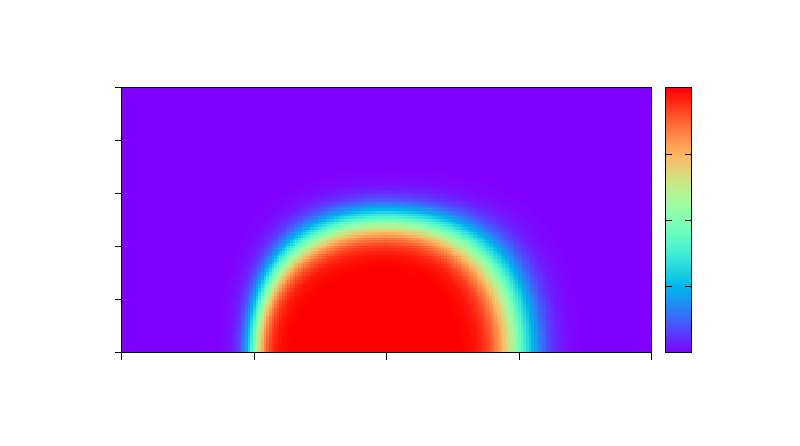
\includegraphics[width={368.50bp},height={198.40bp}]{figures/case_smith_hutton/smith_hutton_N201_Pe1.0e+04}}%
    \gplfronttext
  \end{picture}%
\endgroup
}
% 	% GNUPLOT: LaTeX picture with Postscript
\begingroup
  % Encoding inside the plot.  In the header of your document, this encoding
  % should to defined, e.g., by using
  % \usepackage[cp1252,<other encodings>]{inputenc}
  \inputencoding{cp1252}%
  \makeatletter
  \providecommand\color[2][]{%
    \GenericError{(gnuplot) \space\space\space\@spaces}{%
      Package color not loaded in conjunction with
      terminal option `colourtext'%
    }{See the gnuplot documentation for explanation.%
    }{Either use 'blacktext' in gnuplot or load the package
      color.sty in LaTeX.}%
    \renewcommand\color[2][]{}%
  }%
  \providecommand\includegraphics[2][]{%
    \GenericError{(gnuplot) \space\space\space\@spaces}{%
      Package graphicx or graphics not loaded%
    }{See the gnuplot documentation for explanation.%
    }{The gnuplot epslatex terminal needs graphicx.sty or graphics.sty.}%
    \renewcommand\includegraphics[2][]{}%
  }%
  \providecommand\rotatebox[2]{#2}%
  \@ifundefined{ifGPcolor}{%
    \newif\ifGPcolor
    \GPcolortrue
  }{}%
  \@ifundefined{ifGPblacktext}{%
    \newif\ifGPblacktext
    \GPblacktextfalse
  }{}%
  % define a \g@addto@macro without @ in the name:
  \let\gplgaddtomacro\g@addto@macro
  % define empty templates for all commands taking text:
  \gdef\gplbacktext{}%
  \gdef\gplfronttext{}%
  \makeatother
  \ifGPblacktext
    % no textcolor at all
    \def\colorrgb#1{}%
    \def\colorgray#1{}%
  \else
    % gray or color?
    \ifGPcolor
      \def\colorrgb#1{\color[rgb]{#1}}%
      \def\colorgray#1{\color[gray]{#1}}%
      \expandafter\def\csname LTw\endcsname{\color{white}}%
      \expandafter\def\csname LTb\endcsname{\color{black}}%
      \expandafter\def\csname LTa\endcsname{\color{black}}%
      \expandafter\def\csname LT0\endcsname{\color[rgb]{1,0,0}}%
      \expandafter\def\csname LT1\endcsname{\color[rgb]{0,1,0}}%
      \expandafter\def\csname LT2\endcsname{\color[rgb]{0,0,1}}%
      \expandafter\def\csname LT3\endcsname{\color[rgb]{1,0,1}}%
      \expandafter\def\csname LT4\endcsname{\color[rgb]{0,1,1}}%
      \expandafter\def\csname LT5\endcsname{\color[rgb]{1,1,0}}%
      \expandafter\def\csname LT6\endcsname{\color[rgb]{0,0,0}}%
      \expandafter\def\csname LT7\endcsname{\color[rgb]{1,0.3,0}}%
      \expandafter\def\csname LT8\endcsname{\color[rgb]{0.5,0.5,0.5}}%
    \else
      % gray
      \def\colorrgb#1{\color{black}}%
      \def\colorgray#1{\color[gray]{#1}}%
      \expandafter\def\csname LTw\endcsname{\color{white}}%
      \expandafter\def\csname LTb\endcsname{\color{black}}%
      \expandafter\def\csname LTa\endcsname{\color{black}}%
      \expandafter\def\csname LT0\endcsname{\color{black}}%
      \expandafter\def\csname LT1\endcsname{\color{black}}%
      \expandafter\def\csname LT2\endcsname{\color{black}}%
      \expandafter\def\csname LT3\endcsname{\color{black}}%
      \expandafter\def\csname LT4\endcsname{\color{black}}%
      \expandafter\def\csname LT5\endcsname{\color{black}}%
      \expandafter\def\csname LT6\endcsname{\color{black}}%
      \expandafter\def\csname LT7\endcsname{\color{black}}%
      \expandafter\def\csname LT8\endcsname{\color{black}}%
    \fi
  \fi
    \setlength{\unitlength}{0.0500bp}%
    \ifx\gptboxheight\undefined%
      \newlength{\gptboxheight}%
      \newlength{\gptboxwidth}%
      \newsavebox{\gptboxtext}%
    \fi%
    \setlength{\fboxrule}{0.5pt}%
    \setlength{\fboxsep}{1pt}%
    \definecolor{tbcol}{rgb}{1,1,1}%
\begin{picture}(7370.00,3968.00)%
    \gplgaddtomacro\gplbacktext{%
      \csname LTb\endcsname%%
      \put(814,719){\makebox(0,0)[r]{\strut{}0.0}}%
      \put(814,1234){\makebox(0,0)[r]{\strut{}0.2}}%
      \put(814,1748){\makebox(0,0)[r]{\strut{}0.4}}%
      \put(814,2263){\makebox(0,0)[r]{\strut{}0.6}}%
      \put(814,2777){\makebox(0,0)[r]{\strut{}0.8}}%
      \put(814,3292){\makebox(0,0)[r]{\strut{}1.0}}%
      \put(946,499){\makebox(0,0){\strut{}-1.0}}%
      \put(2233,499){\makebox(0,0){\strut{}-0.5}}%
      \put(3520,499){\makebox(0,0){\strut{}0.0}}%
      \put(4806,499){\makebox(0,0){\strut{}0.5}}%
      \put(6093,499){\makebox(0,0){\strut{}1.0}}%
    }%
    \gplgaddtomacro\gplfronttext{%
      \csname LTb\endcsname%%
      \put(209,2005){\rotatebox{-270}{\makebox(0,0){\strut{}$y \ (\mathrm{m})$}}}%
      \put(3519,169){\makebox(0,0){\strut{}$x \ (\mathrm{m})$}}%
      \csname LTb\endcsname%%
      \put(6611,719){\makebox(0,0)[l]{\strut{}0.0}}%
      \put(6611,1362){\makebox(0,0)[l]{\strut{}0.5}}%
      \put(6611,2005){\makebox(0,0)[l]{\strut{}1.0}}%
      \put(6611,2648){\makebox(0,0)[l]{\strut{}1.5}}%
      \put(6611,3292){\makebox(0,0)[l]{\strut{}2.0}}%
      \put(7073,2005){\rotatebox{-270}{\makebox(0,0){\strut{}$\phi$}}}%
      \put(3519,3622){\makebox(0,0){\strut{}\textbf{Smith--Hutton case} $(\mathrm{Pe} = 10^{4})$}}%
    }%
    \gplbacktext
    \put(0,0){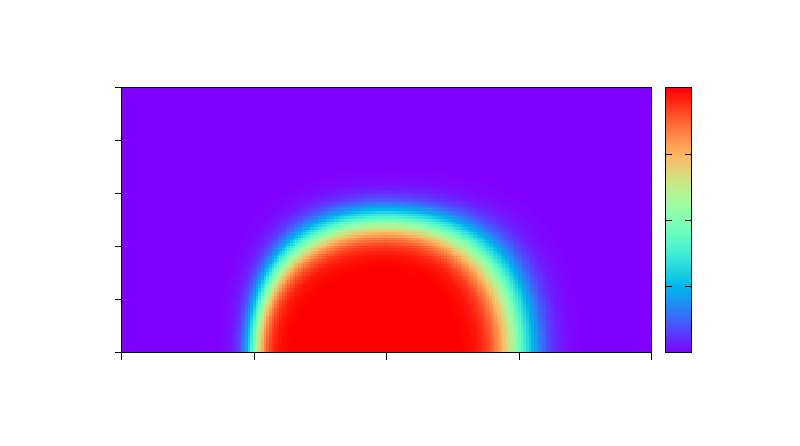
\includegraphics[width={368.50bp},height={198.40bp}]{figures/case_smith_hutton/smith_hutton_N201_Pe1.0e+04}}%
    \gplfronttext
  \end{picture}%
\endgroup

% 	\caption{Numerical solution the the Smith--Hutton case for $\rho / \Gamma = 10^4$.}
% 	\label{fig:smith_hutton_N201_Pe1.0e+04}
% \end{figure}

% \begin{figure}[ht]
% 	\centering
% 	%	\fbox{% GNUPLOT: LaTeX picture with Postscript
\documentclass{minimal}
% Set font size
\makeatletter
\def\@ptsize{1}
\InputIfFileExists{size11.clo}{}{%
   \GenericError{(gnuplot) \space\space\space\@spaces}{%
      Gnuplot Error: File `size11.clo' not found! Could not set font size%
   }{See the gnuplot documentation for explanation.%
   }{For using a font size a file `size<fontsize>.clo' has to exist.
        Falling back ^^Jto default fontsize 10pt.}%
  \def\@ptsize{0}
  \input{size10.clo}%
}%
\makeatother
% Load packages
\usepackage{calc}
\usepackage{graphicx}
\usepackage{color}
\usepackage[cp1252]{inputenc}
\makeatletter
% Select an appropriate default driver (from TeXLive graphics.cfg)
\begingroup
  \chardef\x=0 %
  % check pdfTeX
  \@ifundefined{pdfoutput}{}{%
    \ifcase\pdfoutput
    \else
      \chardef\x=1 %
    \fi
  }%
  % check VTeX
  \@ifundefined{OpMode}{}{%
    \chardef\x=2 %
  }%
\expandafter\endgroup
\ifcase\x
  % default case
  \PassOptionsToPackage{dvips}{geometry}
\or
  % pdfTeX is running in pdf mode
  \PassOptionsToPackage{pdftex}{geometry}
\else
  % VTeX is running
  \PassOptionsToPackage{vtex}{geometry}
\fi
\makeatother
% Set papersize
\usepackage[papersize={368.50bp,198.40bp},text={368.50bp,198.40bp}]{geometry}
% No page numbers and no paragraph indentation
\pagestyle{empty}
\setlength{\parindent}{0bp}%
% Load configuration file
\InputIfFileExists{gnuplot.cfg}{%
  \typeout{Using configuration file gnuplot.cfg}%
}{%
 \typeout{No configuration file gnuplot.cfg found.}%
}%
%
\begin{document}
\begingroup
  % Encoding inside the plot.  In the header of your document, this encoding
  % should to defined, e.g., by using
  % \usepackage[cp1252,<other encodings>]{inputenc}
  \inputencoding{cp1252}%
  \makeatletter
  \providecommand\color[2][]{%
    \GenericError{(gnuplot) \space\space\space\@spaces}{%
      Package color not loaded in conjunction with
      terminal option `colourtext'%
    }{See the gnuplot documentation for explanation.%
    }{Either use 'blacktext' in gnuplot or load the package
      color.sty in LaTeX.}%
    \renewcommand\color[2][]{}%
  }%
  \providecommand\includegraphics[2][]{%
    \GenericError{(gnuplot) \space\space\space\@spaces}{%
      Package graphicx or graphics not loaded%
    }{See the gnuplot documentation for explanation.%
    }{The gnuplot epslatex terminal needs graphicx.sty or graphics.sty.}%
    \renewcommand\includegraphics[2][]{}%
  }%
  \providecommand\rotatebox[2]{#2}%
  \@ifundefined{ifGPcolor}{%
    \newif\ifGPcolor
    \GPcolortrue
  }{}%
  \@ifundefined{ifGPblacktext}{%
    \newif\ifGPblacktext
    \GPblacktextfalse
  }{}%
  % define a \g@addto@macro without @ in the name:
  \let\gplgaddtomacro\g@addto@macro
  % define empty templates for all commands taking text:
  \gdef\gplbacktext{}%
  \gdef\gplfronttext{}%
  \makeatother
  \ifGPblacktext
    % no textcolor at all
    \def\colorrgb#1{}%
    \def\colorgray#1{}%
  \else
    % gray or color?
    \ifGPcolor
      \def\colorrgb#1{\color[rgb]{#1}}%
      \def\colorgray#1{\color[gray]{#1}}%
      \expandafter\def\csname LTw\endcsname{\color{white}}%
      \expandafter\def\csname LTb\endcsname{\color{black}}%
      \expandafter\def\csname LTa\endcsname{\color{black}}%
      \expandafter\def\csname LT0\endcsname{\color[rgb]{1,0,0}}%
      \expandafter\def\csname LT1\endcsname{\color[rgb]{0,1,0}}%
      \expandafter\def\csname LT2\endcsname{\color[rgb]{0,0,1}}%
      \expandafter\def\csname LT3\endcsname{\color[rgb]{1,0,1}}%
      \expandafter\def\csname LT4\endcsname{\color[rgb]{0,1,1}}%
      \expandafter\def\csname LT5\endcsname{\color[rgb]{1,1,0}}%
      \expandafter\def\csname LT6\endcsname{\color[rgb]{0,0,0}}%
      \expandafter\def\csname LT7\endcsname{\color[rgb]{1,0.3,0}}%
      \expandafter\def\csname LT8\endcsname{\color[rgb]{0.5,0.5,0.5}}%
    \else
      % gray
      \def\colorrgb#1{\color{black}}%
      \def\colorgray#1{\color[gray]{#1}}%
      \expandafter\def\csname LTw\endcsname{\color{white}}%
      \expandafter\def\csname LTb\endcsname{\color{black}}%
      \expandafter\def\csname LTa\endcsname{\color{black}}%
      \expandafter\def\csname LT0\endcsname{\color{black}}%
      \expandafter\def\csname LT1\endcsname{\color{black}}%
      \expandafter\def\csname LT2\endcsname{\color{black}}%
      \expandafter\def\csname LT3\endcsname{\color{black}}%
      \expandafter\def\csname LT4\endcsname{\color{black}}%
      \expandafter\def\csname LT5\endcsname{\color{black}}%
      \expandafter\def\csname LT6\endcsname{\color{black}}%
      \expandafter\def\csname LT7\endcsname{\color{black}}%
      \expandafter\def\csname LT8\endcsname{\color{black}}%
    \fi
  \fi
    \setlength{\unitlength}{0.0500bp}%
    \ifx\gptboxheight\undefined%
      \newlength{\gptboxheight}%
      \newlength{\gptboxwidth}%
      \newsavebox{\gptboxtext}%
    \fi%
    \setlength{\fboxrule}{0.5pt}%
    \setlength{\fboxsep}{1pt}%
    \definecolor{tbcol}{rgb}{1,1,1}%
\begin{picture}(7370.00,3968.00)%
    \gplgaddtomacro\gplbacktext{%
      \csname LTb\endcsname%%
      \put(814,733){\makebox(0,0)[r]{\strut{}0.0}}%
      \put(814,1242){\makebox(0,0)[r]{\strut{}0.2}}%
      \put(814,1751){\makebox(0,0)[r]{\strut{}0.4}}%
      \put(814,2260){\makebox(0,0)[r]{\strut{}0.6}}%
      \put(814,2769){\makebox(0,0)[r]{\strut{}0.8}}%
      \put(814,3278){\makebox(0,0)[r]{\strut{}1.0}}%
      \put(1009,513){\makebox(0,0){\strut{}-1.0}}%
      \put(2282,513){\makebox(0,0){\strut{}-0.5}}%
      \put(3554,513){\makebox(0,0){\strut{}0.0}}%
      \put(4827,513){\makebox(0,0){\strut{}0.5}}%
      \put(6099,513){\makebox(0,0){\strut{}1.0}}%
    }%
    \gplgaddtomacro\gplfronttext{%
      \csname LTb\endcsname%%
      \put(209,2005){\rotatebox{-270}{\makebox(0,0){\strut{}$y \ (\mathrm{m})$}}}%
      \put(3554,183){\makebox(0,0){\strut{}$x \ (\mathrm{m})$}}%
      \csname LTb\endcsname%%
      \put(6612,733){\makebox(0,0)[l]{\strut{}0.0}}%
      \put(6612,1369){\makebox(0,0)[l]{\strut{}0.5}}%
      \put(6612,2005){\makebox(0,0)[l]{\strut{}1.0}}%
      \put(6612,2641){\makebox(0,0)[l]{\strut{}1.5}}%
      \put(6612,3278){\makebox(0,0)[l]{\strut{}2.0}}%
      \put(7074,2005){\rotatebox{-270}{\makebox(0,0){\strut{}$\phi$}}}%
      \put(3554,3608){\makebox(0,0){\strut{}\textbf{Smith--Hutton case} $(\rho / \Gamma = 10^{6})$}}%
    }%
    \gplbacktext
    \put(0,0){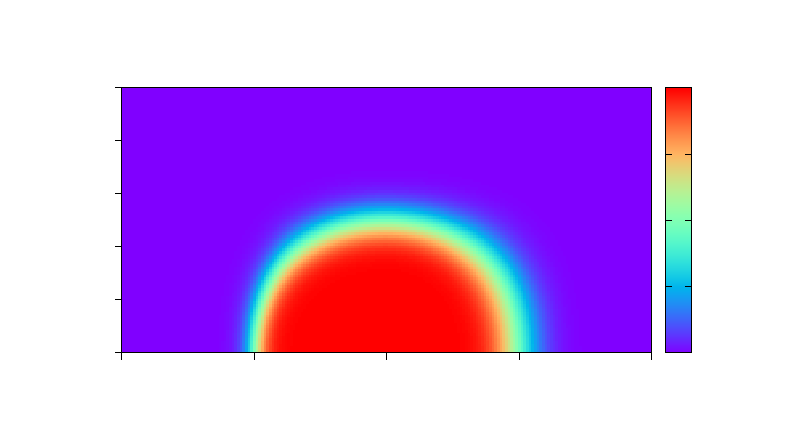
\includegraphics[width={368.50bp},height={198.40bp}]{smith_hutton_N201_Pe1.0e+06-inc}}%
    \gplfronttext
  \end{picture}%
\endgroup
\end{document}
}
% 	% GNUPLOT: LaTeX picture with Postscript
\begingroup
  % Encoding inside the plot.  In the header of your document, this encoding
  % should to defined, e.g., by using
  % \usepackage[cp1252,<other encodings>]{inputenc}
  \inputencoding{cp1252}%
  \makeatletter
  \providecommand\color[2][]{%
    \GenericError{(gnuplot) \space\space\space\@spaces}{%
      Package color not loaded in conjunction with
      terminal option `colourtext'%
    }{See the gnuplot documentation for explanation.%
    }{Either use 'blacktext' in gnuplot or load the package
      color.sty in LaTeX.}%
    \renewcommand\color[2][]{}%
  }%
  \providecommand\includegraphics[2][]{%
    \GenericError{(gnuplot) \space\space\space\@spaces}{%
      Package graphicx or graphics not loaded%
    }{See the gnuplot documentation for explanation.%
    }{The gnuplot epslatex terminal needs graphicx.sty or graphics.sty.}%
    \renewcommand\includegraphics[2][]{}%
  }%
  \providecommand\rotatebox[2]{#2}%
  \@ifundefined{ifGPcolor}{%
    \newif\ifGPcolor
    \GPcolortrue
  }{}%
  \@ifundefined{ifGPblacktext}{%
    \newif\ifGPblacktext
    \GPblacktextfalse
  }{}%
  % define a \g@addto@macro without @ in the name:
  \let\gplgaddtomacro\g@addto@macro
  % define empty templates for all commands taking text:
  \gdef\gplbacktext{}%
  \gdef\gplfronttext{}%
  \makeatother
  \ifGPblacktext
    % no textcolor at all
    \def\colorrgb#1{}%
    \def\colorgray#1{}%
  \else
    % gray or color?
    \ifGPcolor
      \def\colorrgb#1{\color[rgb]{#1}}%
      \def\colorgray#1{\color[gray]{#1}}%
      \expandafter\def\csname LTw\endcsname{\color{white}}%
      \expandafter\def\csname LTb\endcsname{\color{black}}%
      \expandafter\def\csname LTa\endcsname{\color{black}}%
      \expandafter\def\csname LT0\endcsname{\color[rgb]{1,0,0}}%
      \expandafter\def\csname LT1\endcsname{\color[rgb]{0,1,0}}%
      \expandafter\def\csname LT2\endcsname{\color[rgb]{0,0,1}}%
      \expandafter\def\csname LT3\endcsname{\color[rgb]{1,0,1}}%
      \expandafter\def\csname LT4\endcsname{\color[rgb]{0,1,1}}%
      \expandafter\def\csname LT5\endcsname{\color[rgb]{1,1,0}}%
      \expandafter\def\csname LT6\endcsname{\color[rgb]{0,0,0}}%
      \expandafter\def\csname LT7\endcsname{\color[rgb]{1,0.3,0}}%
      \expandafter\def\csname LT8\endcsname{\color[rgb]{0.5,0.5,0.5}}%
    \else
      % gray
      \def\colorrgb#1{\color{black}}%
      \def\colorgray#1{\color[gray]{#1}}%
      \expandafter\def\csname LTw\endcsname{\color{white}}%
      \expandafter\def\csname LTb\endcsname{\color{black}}%
      \expandafter\def\csname LTa\endcsname{\color{black}}%
      \expandafter\def\csname LT0\endcsname{\color{black}}%
      \expandafter\def\csname LT1\endcsname{\color{black}}%
      \expandafter\def\csname LT2\endcsname{\color{black}}%
      \expandafter\def\csname LT3\endcsname{\color{black}}%
      \expandafter\def\csname LT4\endcsname{\color{black}}%
      \expandafter\def\csname LT5\endcsname{\color{black}}%
      \expandafter\def\csname LT6\endcsname{\color{black}}%
      \expandafter\def\csname LT7\endcsname{\color{black}}%
      \expandafter\def\csname LT8\endcsname{\color{black}}%
    \fi
  \fi
    \setlength{\unitlength}{0.0500bp}%
    \ifx\gptboxheight\undefined%
      \newlength{\gptboxheight}%
      \newlength{\gptboxwidth}%
      \newsavebox{\gptboxtext}%
    \fi%
    \setlength{\fboxrule}{0.5pt}%
    \setlength{\fboxsep}{1pt}%
    \definecolor{tbcol}{rgb}{1,1,1}%
\begin{picture}(7370.00,3968.00)%
    \gplgaddtomacro\gplbacktext{%
      \csname LTb\endcsname%%
      \put(814,733){\makebox(0,0)[r]{\strut{}$0$}}%
      \put(814,1242){\makebox(0,0)[r]{\strut{}$0.2$}}%
      \put(814,1751){\makebox(0,0)[r]{\strut{}$0.4$}}%
      \put(814,2260){\makebox(0,0)[r]{\strut{}$0.6$}}%
      \put(814,2769){\makebox(0,0)[r]{\strut{}$0.8$}}%
      \put(814,3278){\makebox(0,0)[r]{\strut{}$1$}}%
      \put(1009,513){\makebox(0,0){\strut{}-1.0}}%
      \put(2282,513){\makebox(0,0){\strut{}-0.5}}%
      \put(3554,513){\makebox(0,0){\strut{}0.0}}%
      \put(4827,513){\makebox(0,0){\strut{}0.5}}%
      \put(6099,513){\makebox(0,0){\strut{}1.0}}%
    }%
    \gplgaddtomacro\gplfronttext{%
      \csname LTb\endcsname%%
      \put(209,2005){\rotatebox{-270}{\makebox(0,0){\strut{}$y \ (\mathrm{m})$}}}%
      \put(3554,183){\makebox(0,0){\strut{}$x \ (\mathrm{m})$}}%
      \csname LTb\endcsname%%
      \put(6612,733){\makebox(0,0)[l]{\strut{}0.0}}%
      \put(6612,1369){\makebox(0,0)[l]{\strut{}0.5}}%
      \put(6612,2005){\makebox(0,0)[l]{\strut{}1.0}}%
      \put(6612,2641){\makebox(0,0)[l]{\strut{}1.5}}%
      \put(6612,3278){\makebox(0,0)[l]{\strut{}2.0}}%
      \put(7074,2005){\rotatebox{-270}{\makebox(0,0){\strut{}$\phi$}}}%
      \put(3554,3608){\makebox(0,0){\strut{}\textbf{Smith--Hutton case} $(\rho / \Gamma = 10^{9})$}}%
    }%
    \gplbacktext
    \put(0,0){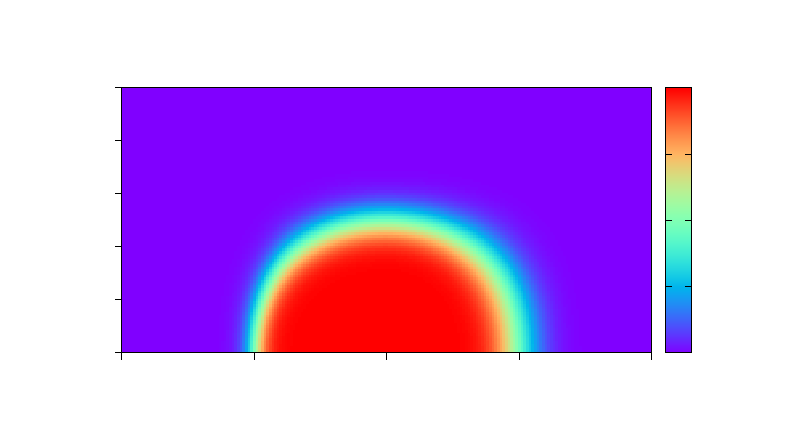
\includegraphics[width={368.50bp},height={198.40bp}]{figures/case_smith_hutton/smith_hutton_N201_Pe1.0e+09}}%
    \gplfronttext
  \end{picture}%
\endgroup

% 	\caption{Numerical solution the the Smith--Hutton case for $\rho / \Gamma = 10^9$.}
% 	\label{fig:smith_hutton_N201_Pe1.0e+09}
% \end{figure}

% /////////////////////////////////////////////////////////////////////////////////////

\clearpage

Figures \ref{fig:smith_hutton_N201_Pe1.0e-01} and
\ref{fig:smith_hutton_N201_Pe1.0e-09} show the solution to the Smith--Hutton
case for $\rho / \Gamma = 10^{-1}$ and $\rho / \Gamma = 10^{-9}$, respectively.
Although a quotient $\rho / \Gamma = 10^{-9}$ implies transport is much weaker
than for $\rho / \Gamma = 10^{-1}$, the differences between both solution are
difficult to detect. The only apparent discrepancy is the central zone of
$\Omega$, where the transitions for $\rho / \Gamma = 10^{-9}$ are much smoother
than for $\rho / \Gamma = 10^{-1}$, which implies transport has lost strength.

\begin{figure}[ht]
	\centering
	%	\fbox{% GNUPLOT: LaTeX picture with Postscript
\begingroup
  % Encoding inside the plot.  In the header of your document, this encoding
  % should to defined, e.g., by using
  % \usepackage[cp1252,<other encodings>]{inputenc}
  \inputencoding{cp1252}%
  \makeatletter
  \providecommand\color[2][]{%
    \GenericError{(gnuplot) \space\space\space\@spaces}{%
      Package color not loaded in conjunction with
      terminal option `colourtext'%
    }{See the gnuplot documentation for explanation.%
    }{Either use 'blacktext' in gnuplot or load the package
      color.sty in LaTeX.}%
    \renewcommand\color[2][]{}%
  }%
  \providecommand\includegraphics[2][]{%
    \GenericError{(gnuplot) \space\space\space\@spaces}{%
      Package graphicx or graphics not loaded%
    }{See the gnuplot documentation for explanation.%
    }{The gnuplot epslatex terminal needs graphicx.sty or graphics.sty.}%
    \renewcommand\includegraphics[2][]{}%
  }%
  \providecommand\rotatebox[2]{#2}%
  \@ifundefined{ifGPcolor}{%
    \newif\ifGPcolor
    \GPcolortrue
  }{}%
  \@ifundefined{ifGPblacktext}{%
    \newif\ifGPblacktext
    \GPblacktextfalse
  }{}%
  % define a \g@addto@macro without @ in the name:
  \let\gplgaddtomacro\g@addto@macro
  % define empty templates for all commands taking text:
  \gdef\gplbacktext{}%
  \gdef\gplfronttext{}%
  \makeatother
  \ifGPblacktext
    % no textcolor at all
    \def\colorrgb#1{}%
    \def\colorgray#1{}%
  \else
    % gray or color?
    \ifGPcolor
      \def\colorrgb#1{\color[rgb]{#1}}%
      \def\colorgray#1{\color[gray]{#1}}%
      \expandafter\def\csname LTw\endcsname{\color{white}}%
      \expandafter\def\csname LTb\endcsname{\color{black}}%
      \expandafter\def\csname LTa\endcsname{\color{black}}%
      \expandafter\def\csname LT0\endcsname{\color[rgb]{1,0,0}}%
      \expandafter\def\csname LT1\endcsname{\color[rgb]{0,1,0}}%
      \expandafter\def\csname LT2\endcsname{\color[rgb]{0,0,1}}%
      \expandafter\def\csname LT3\endcsname{\color[rgb]{1,0,1}}%
      \expandafter\def\csname LT4\endcsname{\color[rgb]{0,1,1}}%
      \expandafter\def\csname LT5\endcsname{\color[rgb]{1,1,0}}%
      \expandafter\def\csname LT6\endcsname{\color[rgb]{0,0,0}}%
      \expandafter\def\csname LT7\endcsname{\color[rgb]{1,0.3,0}}%
      \expandafter\def\csname LT8\endcsname{\color[rgb]{0.5,0.5,0.5}}%
    \else
      % gray
      \def\colorrgb#1{\color{black}}%
      \def\colorgray#1{\color[gray]{#1}}%
      \expandafter\def\csname LTw\endcsname{\color{white}}%
      \expandafter\def\csname LTb\endcsname{\color{black}}%
      \expandafter\def\csname LTa\endcsname{\color{black}}%
      \expandafter\def\csname LT0\endcsname{\color{black}}%
      \expandafter\def\csname LT1\endcsname{\color{black}}%
      \expandafter\def\csname LT2\endcsname{\color{black}}%
      \expandafter\def\csname LT3\endcsname{\color{black}}%
      \expandafter\def\csname LT4\endcsname{\color{black}}%
      \expandafter\def\csname LT5\endcsname{\color{black}}%
      \expandafter\def\csname LT6\endcsname{\color{black}}%
      \expandafter\def\csname LT7\endcsname{\color{black}}%
      \expandafter\def\csname LT8\endcsname{\color{black}}%
    \fi
  \fi
    \setlength{\unitlength}{0.0500bp}%
    \ifx\gptboxheight\undefined%
      \newlength{\gptboxheight}%
      \newlength{\gptboxwidth}%
      \newsavebox{\gptboxtext}%
    \fi%
    \setlength{\fboxrule}{0.5pt}%
    \setlength{\fboxsep}{1pt}%
    \definecolor{tbcol}{rgb}{1,1,1}%
\begin{picture}(7370.00,3968.00)%
    \gplgaddtomacro\gplbacktext{%
      \csname LTb\endcsname%%
      \put(814,719){\makebox(0,0)[r]{\strut{}0.0}}%
      \put(814,1234){\makebox(0,0)[r]{\strut{}0.2}}%
      \put(814,1748){\makebox(0,0)[r]{\strut{}0.4}}%
      \put(814,2263){\makebox(0,0)[r]{\strut{}0.6}}%
      \put(814,2777){\makebox(0,0)[r]{\strut{}0.8}}%
      \put(814,3292){\makebox(0,0)[r]{\strut{}1.0}}%
      \put(946,499){\makebox(0,0){\strut{}-1.0}}%
      \put(2233,499){\makebox(0,0){\strut{}-0.5}}%
      \put(3520,499){\makebox(0,0){\strut{}0.0}}%
      \put(4806,499){\makebox(0,0){\strut{}0.5}}%
      \put(6093,499){\makebox(0,0){\strut{}1.0}}%
    }%
    \gplgaddtomacro\gplfronttext{%
      \csname LTb\endcsname%%
      \put(209,2005){\rotatebox{-270}{\makebox(0,0){\strut{}$y \ (\mathrm{m})$}}}%
      \put(3519,169){\makebox(0,0){\strut{}$x \ (\mathrm{m})$}}%
      \csname LTb\endcsname%%
      \put(6611,719){\makebox(0,0)[l]{\strut{}0.0}}%
      \put(6611,1362){\makebox(0,0)[l]{\strut{}0.5}}%
      \put(6611,2005){\makebox(0,0)[l]{\strut{}1.0}}%
      \put(6611,2648){\makebox(0,0)[l]{\strut{}1.5}}%
      \put(6611,3292){\makebox(0,0)[l]{\strut{}2.0}}%
      \put(7073,2005){\rotatebox{-270}{\makebox(0,0){\strut{}$\phi$}}}%
      \put(3519,3622){\makebox(0,0){\strut{}\textbf{Smith--Hutton case} $(\mathrm{Pe} = 10^{-1})$}}%
    }%
    \gplbacktext
    \put(0,0){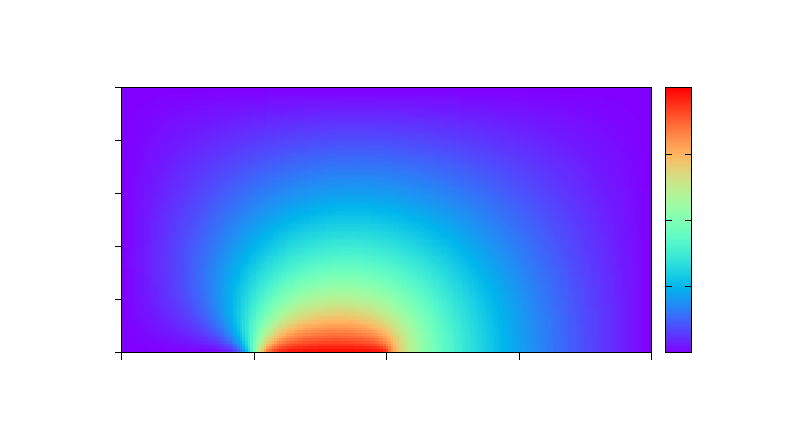
\includegraphics[width={368.50bp},height={198.40bp}]{figures/case_smith_hutton/smith_hutton_N201_Pe1.0e-01}}%
    \gplfronttext
  \end{picture}%
\endgroup
}
	% GNUPLOT: LaTeX picture with Postscript
\begingroup
  % Encoding inside the plot.  In the header of your document, this encoding
  % should to defined, e.g., by using
  % \usepackage[cp1252,<other encodings>]{inputenc}
  \inputencoding{cp1252}%
  \makeatletter
  \providecommand\color[2][]{%
    \GenericError{(gnuplot) \space\space\space\@spaces}{%
      Package color not loaded in conjunction with
      terminal option `colourtext'%
    }{See the gnuplot documentation for explanation.%
    }{Either use 'blacktext' in gnuplot or load the package
      color.sty in LaTeX.}%
    \renewcommand\color[2][]{}%
  }%
  \providecommand\includegraphics[2][]{%
    \GenericError{(gnuplot) \space\space\space\@spaces}{%
      Package graphicx or graphics not loaded%
    }{See the gnuplot documentation for explanation.%
    }{The gnuplot epslatex terminal needs graphicx.sty or graphics.sty.}%
    \renewcommand\includegraphics[2][]{}%
  }%
  \providecommand\rotatebox[2]{#2}%
  \@ifundefined{ifGPcolor}{%
    \newif\ifGPcolor
    \GPcolortrue
  }{}%
  \@ifundefined{ifGPblacktext}{%
    \newif\ifGPblacktext
    \GPblacktextfalse
  }{}%
  % define a \g@addto@macro without @ in the name:
  \let\gplgaddtomacro\g@addto@macro
  % define empty templates for all commands taking text:
  \gdef\gplbacktext{}%
  \gdef\gplfronttext{}%
  \makeatother
  \ifGPblacktext
    % no textcolor at all
    \def\colorrgb#1{}%
    \def\colorgray#1{}%
  \else
    % gray or color?
    \ifGPcolor
      \def\colorrgb#1{\color[rgb]{#1}}%
      \def\colorgray#1{\color[gray]{#1}}%
      \expandafter\def\csname LTw\endcsname{\color{white}}%
      \expandafter\def\csname LTb\endcsname{\color{black}}%
      \expandafter\def\csname LTa\endcsname{\color{black}}%
      \expandafter\def\csname LT0\endcsname{\color[rgb]{1,0,0}}%
      \expandafter\def\csname LT1\endcsname{\color[rgb]{0,1,0}}%
      \expandafter\def\csname LT2\endcsname{\color[rgb]{0,0,1}}%
      \expandafter\def\csname LT3\endcsname{\color[rgb]{1,0,1}}%
      \expandafter\def\csname LT4\endcsname{\color[rgb]{0,1,1}}%
      \expandafter\def\csname LT5\endcsname{\color[rgb]{1,1,0}}%
      \expandafter\def\csname LT6\endcsname{\color[rgb]{0,0,0}}%
      \expandafter\def\csname LT7\endcsname{\color[rgb]{1,0.3,0}}%
      \expandafter\def\csname LT8\endcsname{\color[rgb]{0.5,0.5,0.5}}%
    \else
      % gray
      \def\colorrgb#1{\color{black}}%
      \def\colorgray#1{\color[gray]{#1}}%
      \expandafter\def\csname LTw\endcsname{\color{white}}%
      \expandafter\def\csname LTb\endcsname{\color{black}}%
      \expandafter\def\csname LTa\endcsname{\color{black}}%
      \expandafter\def\csname LT0\endcsname{\color{black}}%
      \expandafter\def\csname LT1\endcsname{\color{black}}%
      \expandafter\def\csname LT2\endcsname{\color{black}}%
      \expandafter\def\csname LT3\endcsname{\color{black}}%
      \expandafter\def\csname LT4\endcsname{\color{black}}%
      \expandafter\def\csname LT5\endcsname{\color{black}}%
      \expandafter\def\csname LT6\endcsname{\color{black}}%
      \expandafter\def\csname LT7\endcsname{\color{black}}%
      \expandafter\def\csname LT8\endcsname{\color{black}}%
    \fi
  \fi
    \setlength{\unitlength}{0.0500bp}%
    \ifx\gptboxheight\undefined%
      \newlength{\gptboxheight}%
      \newlength{\gptboxwidth}%
      \newsavebox{\gptboxtext}%
    \fi%
    \setlength{\fboxrule}{0.5pt}%
    \setlength{\fboxsep}{1pt}%
    \definecolor{tbcol}{rgb}{1,1,1}%
\begin{picture}(7370.00,3968.00)%
    \gplgaddtomacro\gplbacktext{%
      \csname LTb\endcsname%%
      \put(814,719){\makebox(0,0)[r]{\strut{}0.0}}%
      \put(814,1234){\makebox(0,0)[r]{\strut{}0.2}}%
      \put(814,1748){\makebox(0,0)[r]{\strut{}0.4}}%
      \put(814,2263){\makebox(0,0)[r]{\strut{}0.6}}%
      \put(814,2777){\makebox(0,0)[r]{\strut{}0.8}}%
      \put(814,3292){\makebox(0,0)[r]{\strut{}1.0}}%
      \put(946,499){\makebox(0,0){\strut{}-1.0}}%
      \put(2233,499){\makebox(0,0){\strut{}-0.5}}%
      \put(3520,499){\makebox(0,0){\strut{}0.0}}%
      \put(4806,499){\makebox(0,0){\strut{}0.5}}%
      \put(6093,499){\makebox(0,0){\strut{}1.0}}%
    }%
    \gplgaddtomacro\gplfronttext{%
      \csname LTb\endcsname%%
      \put(209,2005){\rotatebox{-270}{\makebox(0,0){\strut{}$y \ (\mathrm{m})$}}}%
      \put(3519,169){\makebox(0,0){\strut{}$x \ (\mathrm{m})$}}%
      \csname LTb\endcsname%%
      \put(6611,719){\makebox(0,0)[l]{\strut{}0.0}}%
      \put(6611,1362){\makebox(0,0)[l]{\strut{}0.5}}%
      \put(6611,2005){\makebox(0,0)[l]{\strut{}1.0}}%
      \put(6611,2648){\makebox(0,0)[l]{\strut{}1.5}}%
      \put(6611,3292){\makebox(0,0)[l]{\strut{}2.0}}%
      \put(7073,2005){\rotatebox{-270}{\makebox(0,0){\strut{}$\phi$}}}%
      \put(3519,3622){\makebox(0,0){\strut{}\textbf{Smith--Hutton case} $(\mathrm{Pe} = 10^{-1})$}}%
    }%
    \gplbacktext
    \put(0,0){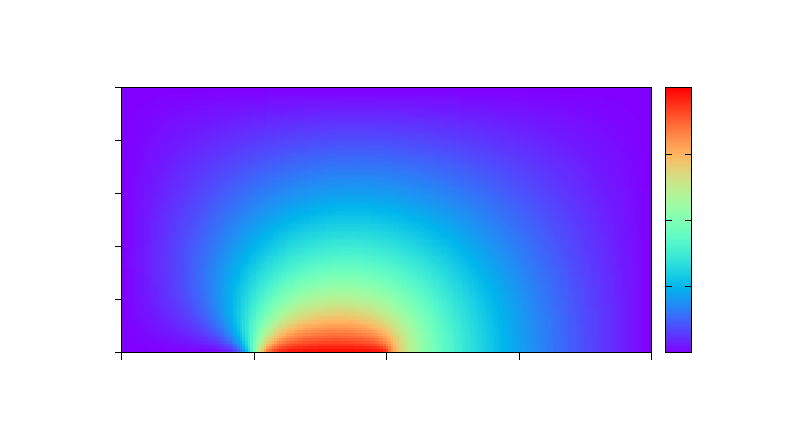
\includegraphics[width={368.50bp},height={198.40bp}]{figures/case_smith_hutton/smith_hutton_N201_Pe1.0e-01}}%
    \gplfronttext
  \end{picture}%
\endgroup

	\caption{Numerical solution the the Smith--Hutton case for $\rho / \Gamma = 10^{-1}$.}
	\label{fig:smith_hutton_N201_Pe1.0e-01}
	\vspace{1cm}
	% GNUPLOT: LaTeX picture with Postscript
\begingroup
  % Encoding inside the plot.  In the header of your document, this encoding
  % should to defined, e.g., by using
  % \usepackage[cp1252,<other encodings>]{inputenc}
  \inputencoding{cp1252}%
  \makeatletter
  \providecommand\color[2][]{%
    \GenericError{(gnuplot) \space\space\space\@spaces}{%
      Package color not loaded in conjunction with
      terminal option `colourtext'%
    }{See the gnuplot documentation for explanation.%
    }{Either use 'blacktext' in gnuplot or load the package
      color.sty in LaTeX.}%
    \renewcommand\color[2][]{}%
  }%
  \providecommand\includegraphics[2][]{%
    \GenericError{(gnuplot) \space\space\space\@spaces}{%
      Package graphicx or graphics not loaded%
    }{See the gnuplot documentation for explanation.%
    }{The gnuplot epslatex terminal needs graphicx.sty or graphics.sty.}%
    \renewcommand\includegraphics[2][]{}%
  }%
  \providecommand\rotatebox[2]{#2}%
  \@ifundefined{ifGPcolor}{%
    \newif\ifGPcolor
    \GPcolortrue
  }{}%
  \@ifundefined{ifGPblacktext}{%
    \newif\ifGPblacktext
    \GPblacktextfalse
  }{}%
  % define a \g@addto@macro without @ in the name:
  \let\gplgaddtomacro\g@addto@macro
  % define empty templates for all commands taking text:
  \gdef\gplbacktext{}%
  \gdef\gplfronttext{}%
  \makeatother
  \ifGPblacktext
    % no textcolor at all
    \def\colorrgb#1{}%
    \def\colorgray#1{}%
  \else
    % gray or color?
    \ifGPcolor
      \def\colorrgb#1{\color[rgb]{#1}}%
      \def\colorgray#1{\color[gray]{#1}}%
      \expandafter\def\csname LTw\endcsname{\color{white}}%
      \expandafter\def\csname LTb\endcsname{\color{black}}%
      \expandafter\def\csname LTa\endcsname{\color{black}}%
      \expandafter\def\csname LT0\endcsname{\color[rgb]{1,0,0}}%
      \expandafter\def\csname LT1\endcsname{\color[rgb]{0,1,0}}%
      \expandafter\def\csname LT2\endcsname{\color[rgb]{0,0,1}}%
      \expandafter\def\csname LT3\endcsname{\color[rgb]{1,0,1}}%
      \expandafter\def\csname LT4\endcsname{\color[rgb]{0,1,1}}%
      \expandafter\def\csname LT5\endcsname{\color[rgb]{1,1,0}}%
      \expandafter\def\csname LT6\endcsname{\color[rgb]{0,0,0}}%
      \expandafter\def\csname LT7\endcsname{\color[rgb]{1,0.3,0}}%
      \expandafter\def\csname LT8\endcsname{\color[rgb]{0.5,0.5,0.5}}%
    \else
      % gray
      \def\colorrgb#1{\color{black}}%
      \def\colorgray#1{\color[gray]{#1}}%
      \expandafter\def\csname LTw\endcsname{\color{white}}%
      \expandafter\def\csname LTb\endcsname{\color{black}}%
      \expandafter\def\csname LTa\endcsname{\color{black}}%
      \expandafter\def\csname LT0\endcsname{\color{black}}%
      \expandafter\def\csname LT1\endcsname{\color{black}}%
      \expandafter\def\csname LT2\endcsname{\color{black}}%
      \expandafter\def\csname LT3\endcsname{\color{black}}%
      \expandafter\def\csname LT4\endcsname{\color{black}}%
      \expandafter\def\csname LT5\endcsname{\color{black}}%
      \expandafter\def\csname LT6\endcsname{\color{black}}%
      \expandafter\def\csname LT7\endcsname{\color{black}}%
      \expandafter\def\csname LT8\endcsname{\color{black}}%
    \fi
  \fi
    \setlength{\unitlength}{0.0500bp}%
    \ifx\gptboxheight\undefined%
      \newlength{\gptboxheight}%
      \newlength{\gptboxwidth}%
      \newsavebox{\gptboxtext}%
    \fi%
    \setlength{\fboxrule}{0.5pt}%
    \setlength{\fboxsep}{1pt}%
    \definecolor{tbcol}{rgb}{1,1,1}%
\begin{picture}(7370.00,3968.00)%
    \gplgaddtomacro\gplbacktext{%
      \csname LTb\endcsname%%
      \put(814,733){\makebox(0,0)[r]{\strut{}$0$}}%
      \put(814,1242){\makebox(0,0)[r]{\strut{}$0.2$}}%
      \put(814,1751){\makebox(0,0)[r]{\strut{}$0.4$}}%
      \put(814,2260){\makebox(0,0)[r]{\strut{}$0.6$}}%
      \put(814,2769){\makebox(0,0)[r]{\strut{}$0.8$}}%
      \put(814,3278){\makebox(0,0)[r]{\strut{}$1$}}%
      \put(1009,513){\makebox(0,0){\strut{}-1.0}}%
      \put(2282,513){\makebox(0,0){\strut{}-0.5}}%
      \put(3554,513){\makebox(0,0){\strut{}0.0}}%
      \put(4827,513){\makebox(0,0){\strut{}0.5}}%
      \put(6099,513){\makebox(0,0){\strut{}1.0}}%
    }%
    \gplgaddtomacro\gplfronttext{%
      \csname LTb\endcsname%%
      \put(209,2005){\rotatebox{-270}{\makebox(0,0){\strut{}$y \ (\mathrm{m})$}}}%
      \put(3554,183){\makebox(0,0){\strut{}$x \ (\mathrm{m})$}}%
      \csname LTb\endcsname%%
      \put(6612,733){\makebox(0,0)[l]{\strut{}0.0}}%
      \put(6612,1369){\makebox(0,0)[l]{\strut{}0.5}}%
      \put(6612,2005){\makebox(0,0)[l]{\strut{}1.0}}%
      \put(6612,2641){\makebox(0,0)[l]{\strut{}1.5}}%
      \put(6612,3278){\makebox(0,0)[l]{\strut{}2.0}}%
      \put(7074,2005){\rotatebox{-270}{\makebox(0,0){\strut{}$\phi$}}}%
      \put(3554,3608){\makebox(0,0){\strut{}\textbf{Smith--Hutton case} $(\rho / \Gamma = 10^{-9})$}}%
    }%
    \gplbacktext
    \put(0,0){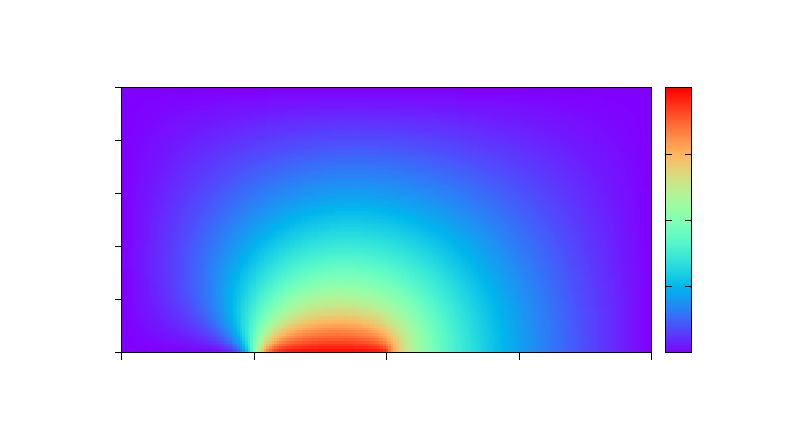
\includegraphics[width={368.50bp},height={198.40bp}]{figures/case_smith_hutton/smith_hutton_N201_Pe1.0e-09}}%
    \gplfronttext
  \end{picture}%
\endgroup

	\caption{Numerical solution the the Smith--Hutton case for $\rho / \Gamma = 10^{-9}$.}
	\label{fig:smith_hutton_N201_Pe1.0e-09}
\end{figure}




